% SQL2Mongo: Phase 3 Final Project Report
% Build: xelatex SQL2Mongo_Report.tex  (run twice so the contents page and figure numbers update)
\documentclass[12pt,a4paper]{report}

\usepackage{fontspec}
\setmainfont{Times New Roman}
\setmonofont{Consolas}[Scale=0.9]

\usepackage[a4paper,margin=2.54cm]{geometry}
\usepackage{setspace}
\setstretch{1.15}
\usepackage{titlesec}
\usepackage{tabularx,longtable,array}
\usepackage{enumitem}
\usepackage{caption}
\usepackage{float}
\usepackage{needspace}
\usepackage{fancyvrb}
\usepackage{listings}
\usepackage{graphicx}
\usepackage{tikz}
\usetikzlibrary{positioning,arrows.meta,calc}
\usepackage{xurl}
\usepackage[hidelinks]{hyperref}
\urlstyle{same}
\graphicspath{{figures/}}
\usepackage{etoolbox}
\makeatletter
\patchcmd{\chapter}{\if@openright\cleardoublepage\else\clearpage\fi}{\par\vspace{16pt}}{}{}
\makeatother

% Headings: "Chapter 1: Introduction", then "1.1 Background"
\titleformat{\chapter}[hang]{\normalfont\Large\bfseries}{\chaptertitlename\ \thechapter:}{0.4em}{}
\titlespacing*{\chapter}{0pt}{4pt}{12pt}
\titleformat{\section}{\normalfont\large\bfseries}{\thesection}{0.6em}{}
\titlespacing*{\section}{0pt}{14pt}{6pt}
\titleformat{\subsection}{\normalfont\normalsize\bfseries}{}{0em}{}
\titlespacing*{\subsection}{0pt}{10pt}{4pt}
\setcounter{secnumdepth}{1}
\setcounter{tocdepth}{0}

\pagestyle{plain}
\setlist{itemsep=2pt, topsep=4pt}
\captionsetup{labelfont=bf, skip=6pt}
\renewcommand{\arraystretch}{1.3}
\newcolumntype{L}{>{\raggedright\arraybackslash}X}
\newcolumntype{P}[1]{>{\raggedright\arraybackslash}p{#1}}
\setlength{\emergencystretch}{3em}

% Inline code (allows line breaks after underscores)
\newcommand{\codeus}{\textunderscore\allowbreak}
\DeclareRobustCommand{\code}[1]{\texttt{\let\_\codeus #1}}

% Code and program output
\lstset{basicstyle=\ttfamily\small\setstretch{1.0}, frame=single, framesep=4pt,
  xleftmargin=3pt, xrightmargin=3pt, columns=fullflexible, keepspaces=true,
  breaklines=true, showstringspaces=false, aboveskip=8pt, belowskip=8pt}
\fvset{fontsize=\small, baselinestretch=1, frame=single, framesep=4pt, xleftmargin=3pt, xrightmargin=3pt}

\begin{document}

% ---------------------------------------------------------------------
% Title page
% ---------------------------------------------------------------------
\begin{titlepage}
\centering
\setstretch{1.25}
\vspace*{2.2cm}
{\fontsize{30}{36}\selectfont\bfseries SQL2Mongo\par}
\vspace{0.5cm}
{\normalsize GitHub Link: \url{https://github.com/71percentbanana/MQL}\par}
\vspace{1.4cm}
{\Large A SQL-to-MongoDB Query Compiler and Execution Engine\par}
\vspace{1.6cm}
{\large\bfseries Phase 3: Final Project Report\par}
\vspace{2.6cm}
{\large BCSE307L / BCSE307P: Compiler Design and Compiler Design Lab\par}
\vspace{1.4cm}
{\large Submitted by: Alan James\par}
{\large Registration Number: 24BCT0181\par}
\vfill
{\large School of Computer Science and Engineering, VIT Vellore\par}
{\large Fall Semester 2026--27\par}
\vspace{0.6cm}
{\large October 2026\par}
\end{titlepage}

% ---------------------------------------------------------------------
% Abstract and contents
% ---------------------------------------------------------------------
\pagenumbering{roman}
\chapter*{Abstract}
\addcontentsline{toc}{chapter}{Abstract}

Most developers learn SQL before they ever work with MongoDB, and moving to MongoDB means relearning how to write the same queries in a very different language. SQL2Mongo addresses this. It is a source-to-source compiler, written in C, that translates SQL \code{SELECT} queries into MongoDB aggregation pipelines and runs them against document collections stored as JSON files.

The compiler implements seven phases: lexical analysis, recursive-descent parsing with parse-tree and AST output, symbol-table-driven semantic analysis, intermediate code in three-address code, quadruple and triple form, an optimization pass, MongoDB Query Language (MQL) code generation, and execution. Each phase can be shown on its own through a command-line flag, and a local web dashboard presents the same output page by page.

The supported language covers projections, \code{WHERE} filters with \code{AND}, \code{OR} and parentheses, six comparison operators, \code{ORDER BY} and \code{LIMIT}. The compiler is 2,456 lines of C in ten modules and uses only the C standard library. Of 21 test queries covering valid, boundary and erroneous input, 19 behave exactly as expected; the remaining 2 expose limitations in the generated target code, which are documented with their fixes. All 9 automated integration tests pass.

\clearpage
\tableofcontents
\clearpage

% ---------------------------------------------------------------------
% Phase 3 overview
% ---------------------------------------------------------------------
\chapter*{Phase 3 Overview}
\addcontentsline{toc}{chapter}{Phase 3 Overview}
The objective of Phase 3 is to complete the project, integrate all modules and validate the final system. Phase 1 defined the query language and produced the lexer and parser. Phase 2 added the symbol table, semantic checks, the abstract syntax tree and three-address code. Phase 3 adds the following:
\begin{itemize}
  \item \textbf{Complete intermediate representation.} Quadruples and triples are generated alongside three-address code.
  \item \textbf{Back end.} An optimization pass and a code generator that emits a MongoDB aggregation pipeline for every valid query.
  \item \textbf{Execution on real data files.} An execution engine runs the compiled query against collections stored as JSON files in \code{data/}, in the same format that \code{mongoexport -{}-jsonArray} produces. Editing a file changes the results of the next query without rebuilding.
  \item \textbf{Web dashboard.} A local web interface with three pages: Query (SQL in, MongoDB pipeline and documents out), Compiler phases (the output of all seven phases), and Database (the contents of each collection file).
  \item \textbf{Validation.} 21 test queries, including two new execution-error cases, and 9 automated integration tests that run the real executable.
\end{itemize}

\cleardoublepage
\pagenumbering{arabic}

% =====================================================================
\chapter{Introduction}
% =====================================================================
SQL2Mongo lets someone who already knows SQL write a query in SQL and get the equivalent MongoDB query. It does this by applying the full compiler pipeline to the two languages, with SQL as the source and the MongoDB Query Language (MQL) as the target.

\section{Background}
Relational databases are queried with SQL, a declarative language with a fixed keyword grammar. Document databases such as MongoDB store JSON-like documents and are queried with MQL, where a query is itself a JSON structure. MongoDB's aggregation framework expresses a query as a pipeline of stages such as \code{\$match}, \code{\$sort}, \code{\$limit} and \code{\$project} \cite{mongo-pipeline}.

Both languages describe the same operations, but with different syntax and structure, so moving a query from one to the other is a translation problem.

\section{Motivation}
Most students and developers learn SQL first. It is what database courses teach, and it is the language people reach for when they think about querying data. Many of them later work on projects that use MongoDB, and they then have to learn a second, very different way of writing the same queries.

I faced this myself during my internship, where the project used MongoDB. I already knew how to write the queries I needed in SQL, but I had to work out how to express each one in MongoDB: which operator replaces \code{>=}, how \code{AND} and \code{OR} turn into nested \code{\$and} and \code{\$or} arrays, and in what order the pipeline stages must go. A small mistake in this translation does not raise an error. The query simply returns the wrong documents, or none at all.

This project grew out of that experience. Translating one query language into another is exactly what a compiler does, so I built one that takes the SQL a developer already knows and produces the equivalent MongoDB query. Because every phase prints its output, the tool also shows how each part of the SQL query maps to MongoDB, which helps someone who is learning MongoDB as well as someone who only needs the translated query.

\section{Problem Area}
The project sits in source-to-source compilation (transpilation) and database query processing. It combines classic front-end phases (scanning, parsing, semantic checks) with query-processing ideas (relational operators, query plans, predicate pushdown).

\section{Summary of the Three Phases}
\begin{table}[H]
\centering\small
\begin{tabularx}{\linewidth}{|P{2.2cm}|L|}
\hline
\textbf{Phase} & \textbf{Result} \\ \hline
Phase 1 & Query language and grammar, lexer with token table, recursive-descent parser with a validity check. \\ \hline
Phase 2 & Symbol table and semantic checks, abstract syntax tree, three-address code. \\ \hline
Phase 3 & Quadruples and triples, optimizer, MQL code generator, execution engine over JSON collection files, web dashboard, and the full test suite. \\ \hline
\end{tabularx}
\caption{What each phase of the project delivered}
\end{table}

% =====================================================================
\chapter{Problem Statement}
% =====================================================================
A developer who knows SQL but has to work with MongoDB must translate every query by hand. The problem this project solves is: given a SQL \code{SELECT} query over a known schema, produce an equivalent and valid MongoDB aggregation pipeline, or report exactly where and why the query is invalid.

Hand translation from SQL to MQL has three recurring failure points:
\begin{itemize}
  \item \textbf{Operator mapping.} Each SQL comparison has a different MQL spelling (\code{>=} to \code{\$gte}, \code{!=} and \code{<>} to \code{\$ne}), and equality is written without an operator.
  \item \textbf{Logical structure.} Operator precedence must be preserved: \code{a AND b OR c} means \code{(a AND b) OR c}, which becomes an \code{\$or} array containing an \code{\$and} array.
  \item \textbf{Schema errors found late.} A misspelled field or a string compared with a number is not rejected by MongoDB. The query simply returns no documents, so the mistake goes unnoticed.
\end{itemize}
The translator must therefore check queries before generating code, its diagnostics must point to the line and column of the fault, and its output must be verifiable by running the query on real documents.

\section{Requirements}
\begin{table}[H]
\centering\small
\begin{tabularx}{\linewidth}{|P{2.6cm}|L|}
\hline
\textbf{Type} & \textbf{Requirement} \\ \hline
Input & A SQL query, either as a \code{.sql} file path or as an inline string on the command line, or typed into the web dashboard. \\ \hline
Data & Collections stored as JSON arrays of flat documents, one file per collection in \code{data/}. \\ \hline
Output & Token table, parse tree, AST, symbol table, TAC, quadruples, triples, optimization report, MQL pipeline and query results, each selectable by a flag. \\ \hline
Functional & Reject lexical, syntax and semantic errors with a message giving the line, column and expected construct. \\ \hline
Functional & Return exit code 0 on success, 1 on a lexical or syntax error, 2 on a semantic error and 3 when a collection file is missing or invalid, so tests can be automated. \\ \hline
Interface & A local web page that shows the SQL, the generated pipeline, the result documents, every compiler phase and the stored collections. \\ \hline
System & Any machine with a C compiler; Node.js 20 or newer for the dashboard. No database server or third-party library is needed. \\ \hline
\end{tabularx}
\caption{System requirements}
\end{table}

% =====================================================================
\chapter{Objectives}
% =====================================================================
Each objective set at the start of the project is listed with its status and the place in this report where the evidence can be found.

{\small
\setlength{\tabcolsep}{4pt}
\begin{longtable}{|>{\raggedright\arraybackslash}p{0.6cm}|>{\raggedright\arraybackslash}p{8.0cm}|>{\raggedright\arraybackslash}p{1.3cm}|>{\raggedright\arraybackslash}p{4.4cm}|}
\caption{Objectives, status and evidence}\\
\hline
\textbf{No.} & \textbf{Objective} & \textbf{Status} & \textbf{Evidence} \\ \hline
\endfirsthead
\hline
\textbf{No.} & \textbf{Objective} & \textbf{Status} & \textbf{Evidence} \\ \hline
\endhead
1 & Build a lexical analyser that recognises 11 SQL keywords, identifiers, number and string literals, 7 comparison lexemes and 5 delimiters, skips comments, and tracks line and column. & Done & Section 7.2, \code{sql\_lexer.c} \\ \hline
2 & Build a recursive-descent parser that prints a concrete parse tree and builds an abstract syntax tree. & Done & Sections 7.3 and 7.4 \\ \hline
3 & Build a symbol table of collections and typed fields, and use it to check collections, fields and types. & Done & Section 7.5 \\ \hline
4 & Generate intermediate code as three-address code, quadruples and triples. & Done & Section 7.6 \\ \hline
5 & Apply query optimizations: predicate pushdown and projection pruning. & Done & Section 7.7 \\ \hline
6 & Generate target MQL as a \code{db.<collection>.\allowbreak aggregate([...])} pipeline. & Done & Section 7.8 \\ \hline
7 & Execute the compiled query on documents loaded from JSON collection files. & Done & Sections 7.9 and 8.4 \\ \hline
8 & Provide a web interface that shows the result and every compiler phase. & Done & Section 8.5, Figures 9.3--9.5 \\ \hline
9 & Validate the system with valid, invalid, boundary and complex test queries and automated tests. & Done & Chapter 9 \\ \hline
\end{longtable}
}

\section{Scope}
\textbf{In scope:} single-collection \code{SELECT} queries with a column list or \code{*}; \code{WHERE} with \code{=}, \code{!=}, \code{<>}, \code{>}, \code{>=}, \code{<}, \code{<=}, \code{AND}, \code{OR} and parentheses; \code{ORDER BY} on one field, \code{ASC} or \code{DESC}; \code{LIMIT}; case-insensitive keywords; flat JSON documents with string and number values.

\textbf{Out of scope:} \code{JOIN}, \code{GROUP BY} and aggregate functions, subqueries, \code{IN}, \code{LIKE} and \code{BETWEEN}, data-changing statements (\code{INSERT}, \code{UPDATE}, \code{DELETE}), nested documents and arrays, and a connection to a MongoDB server. \code{NOT} is recognised by the lexer as a reserved word but is not yet part of the grammar.

% =====================================================================
\chapter{Background Study}
% =====================================================================
SQL-to-MQL translators already exist, but they hide their internals behind a product or a third-party parser. SQL2Mongo builds every phase by hand so each one can be shown and explained.

\section{Existing Approaches}
\begin{table}[H]
\centering\small
\begin{tabularx}{\linewidth}{|P{3.4cm}|L|L|}
\hline
\textbf{Approach} & \textbf{How it works} & \textbf{Difference from SQL2Mongo} \\ \hline
MongoDB SQL to Aggregation Mapping Chart \cite{mongo-chart} & Official reference table that maps SQL clauses to pipeline stages. & A manual guide; it performs no translation or checking. \\ \hline
mongotranslate, MongoDB BI Connector \cite{mongotranslate} & Command-line tool that shows how a SQL query is expressed as an aggregation pipeline, using a schema (DRDL) file. & Part of a large commercial product; its phases are not visible. \\ \hline
sql-to-mongo-db-query-converter \cite{russell} & Java library that converts SQL into MongoDB find, update, delete and aggregation queries. & Parsing is delegated to the JSqlParser library, so there is no hand-built lexer or parser. \\ \hline
SQL2Mongo (this project) & Hand-written lexer, parser, semantic analyser, IR generator, optimizer, code generator and executor in C. & Every phase prints its own output; schema errors are caught before code generation. \\ \hline
\end{tabularx}
\caption{Comparison with existing SQL-to-MongoDB translators}
\end{table}

\section{SQL-to-MQL Mapping}
The target forms follow MongoDB's own mapping chart \cite{mongo-chart}.
\begin{table}[H]
\centering\small
\begin{tabular}{|l|l|}
\hline
\textbf{SQL construct} & \textbf{MQL stage or operator} \\ \hline
\code{FROM t} & \code{db.t.aggregate([...])} \\ \hline
\code{WHERE} & \code{\$match} \\ \hline
\code{ORDER BY f ASC} / \code{DESC} & \code{\$sort: \{ f: 1 \}} / \code{\{ f: -1 \}} \\ \hline
\code{LIMIT n} & \code{\$limit: n} \\ \hline
\code{SELECT a, b} & \code{\$project: \{ \_id: 0, a: 1, b: 1 \}} \\ \hline
\code{SELECT *} & no \code{\$project} stage \\ \hline
\code{=} & implicit equality \code{\{ f: v \}} \\ \hline
\code{!=}, \code{<>}, \code{>}, \code{>=}, \code{<}, \code{<=} & \code{\$ne}, \code{\$ne}, \code{\$gt}, \code{\$gte}, \code{\$lt}, \code{\$lte} \\ \hline
\code{AND}, \code{OR} & \code{\$and: [...]}, \code{\$or: [...]} \\ \hline
\end{tabular}
\caption{SQL constructs and their MQL equivalents}
\end{table}

\section{Compiler Techniques Used}
\begin{itemize}
  \item \textbf{Phases of a compiler.} The project follows the analysis--synthesis model of Aho, Lam, Sethi and Ullman \cite{aho}: scanning, parsing, semantic analysis, intermediate code, optimization and code generation.
  \item \textbf{Recursive-descent parsing.} One function per non-terminal; operator precedence is encoded by grammar layering (\code{OR} below \code{AND} below comparisons).
  \item \textbf{Symbol tables and type checking.} The schema catalog acts as a symbol table holding each field's name and type.
  \item \textbf{Intermediate representations.} Three-address code, quadruples and triples, with relational-algebra operators \cite{codd} (scan, filter, sort, limit, project) as the instruction set.
  \item \textbf{Query optimization.} Filtering early (predicate pushdown) is a standard relational technique \cite{selinger}. MongoDB's pipeline optimization guide \cite{mongo-opt} also moves \code{\$match} ahead of \code{\$sort} and keeps \code{\$project} last.
\end{itemize}

\section{The Collection File Format}
MongoDB's \code{mongoexport} tool writes a collection as JSON; with the \code{-{}-jsonArray} option the output is a single array of documents \cite{mongoexport}. SQL2Mongo stores each collection in exactly this form, using the JSON grammar of RFC 8259 \cite{json}. The files can therefore be imported into a real MongoDB server unchanged with \code{mongoimport -{}-jsonArray}, and the generated pipelines can be run against the same data.

\section{Technology Selection}
C was chosen from the course's recommended languages because it forces every data structure to be explicit \cite{kr}. The lexer, parser and JSON reader are written by hand rather than with Flex, Bison or a JSON library, so the scanning and parsing algorithms are visible in the source. The dashboard uses Node.js with no third-party packages, because it only needs to start the compiler and serve three static files. Development used GCC (MinGW 6.3.0), Visual Studio Code and Git.

% =====================================================================
\chapter{System Design}
% =====================================================================
SQL2Mongo is a single-pass pipeline of seven phases. The parser builds one AST, and every later phase reads it. A separate web layer runs the compiler and displays its output.

\section{Architecture}
\begin{figure}[H]
\centering
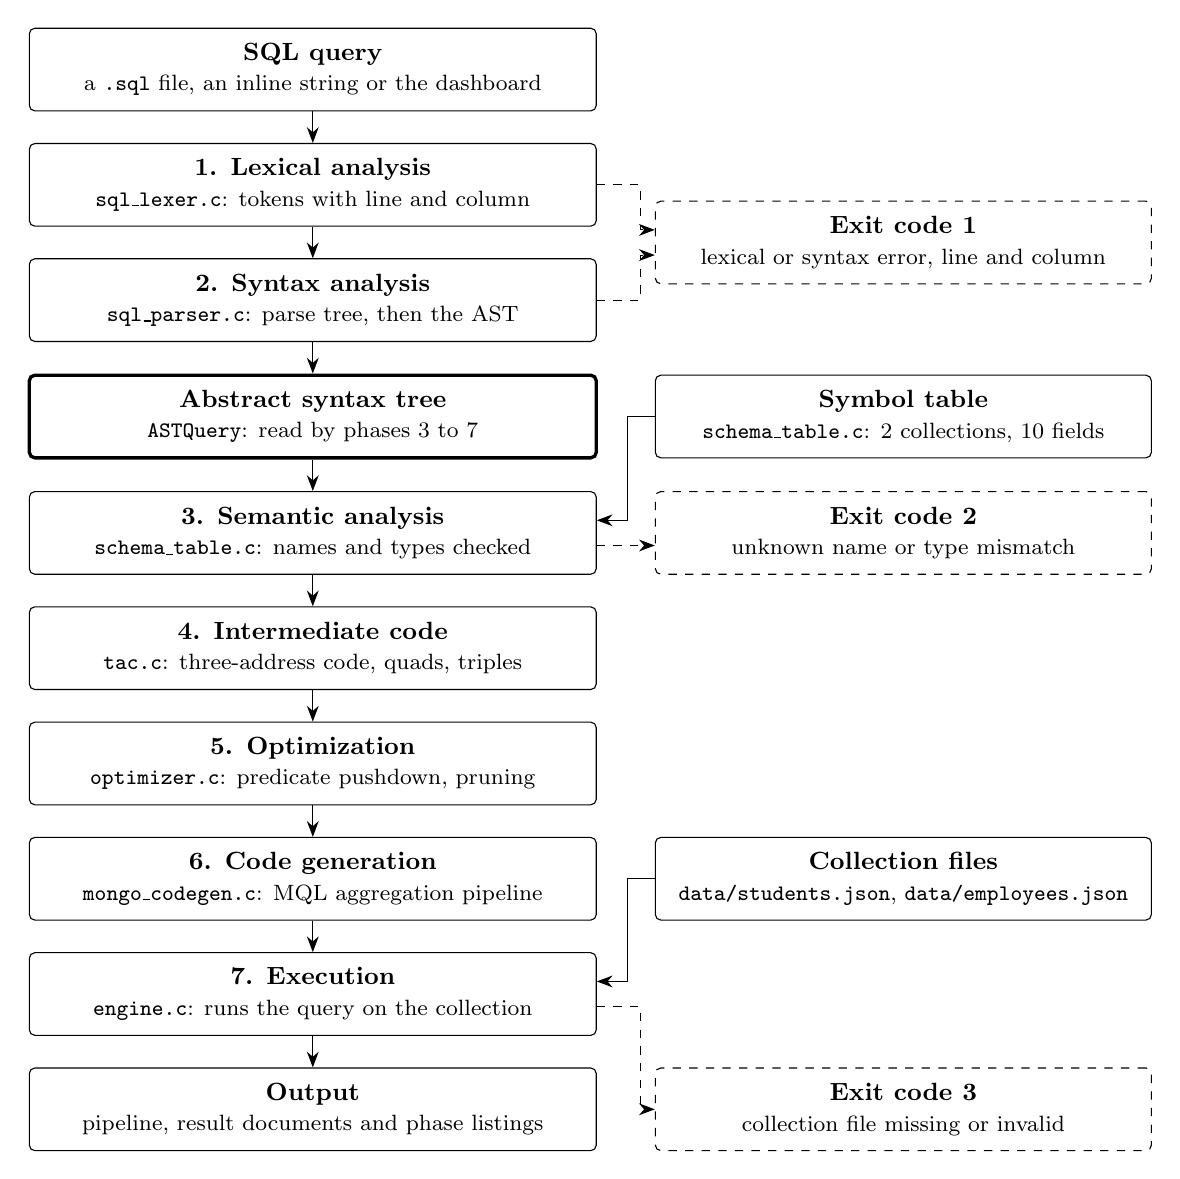
\begin{tikzpicture}[
  node distance=4mm,
  phase/.style={draw, rounded corners=2pt, minimum width=7.2cm, minimum height=1.05cm, align=center, inner sep=3pt},
  astn/.style={phase, line width=1.2pt},
  side/.style={phase, minimum width=6.3cm},
  errn/.style={side, dashed},
  flow/.style={-{Stealth[length=2mm]}},
  errflow/.style={-{Stealth[length=2mm]}, dashed},
]
\newcommand{\nm}[1]{{\small\bfseries #1}}
\newcommand{\bd}[1]{{\footnotesize #1}}
\node[phase] (in) {\nm{SQL query}\\[-1pt]\bd{a \code{.sql} file, an inline string or the dashboard}};
\node[phase, below=of in] (lex) {\nm{1. Lexical analysis}\\[-1pt]\bd{\code{sql\_lexer.c}: tokens with line and column}};
\node[phase, below=of lex] (par) {\nm{2. Syntax analysis}\\[-1pt]\bd{\code{sql\_parser.c}: parse tree, then the AST}};
\node[astn, below=of par] (ast) {\nm{Abstract syntax tree}\\[-1pt]\bd{\code{ASTQuery}: read by phases 3 to 7}};
\node[phase, below=of ast] (sem) {\nm{3. Semantic analysis}\\[-1pt]\bd{\code{schema\_table.c}: names and types checked}};
\node[phase, below=of sem] (ir) {\nm{4. Intermediate code}\\[-1pt]\bd{\code{tac.c}: three-address code, quads, triples}};
\node[phase, below=of ir] (opt) {\nm{5. Optimization}\\[-1pt]\bd{\code{optimizer.c}: predicate pushdown, pruning}};
\node[phase, below=of opt] (cg) {\nm{6. Code generation}\\[-1pt]\bd{\code{mongo\_codegen.c}: MQL aggregation pipeline}};
\node[phase, below=of cg] (exe) {\nm{7. Execution}\\[-1pt]\bd{\code{engine.c}: runs the query on the collection}};
\node[phase, below=of exe] (out) {\nm{Output}\\[-1pt]\bd{pipeline, result documents and phase listings}};
\node[errn] (e1) at ($(lex)!0.5!(par) + (7.5cm,0)$) {\nm{Exit code 1}\\[-1pt]\bd{lexical or syntax error, line and column}};
\node[side] (sym) at ($(ast) + (7.5cm,0)$) {\nm{Symbol table}\\[-1pt]\bd{\code{schema\_table.c}: 2 collections, 10 fields}};
\node[errn] (e2) at ($(sem) + (7.5cm,0)$) {\nm{Exit code 2}\\[-1pt]\bd{unknown name or type mismatch}};
\node[side] (data) at ($(cg) + (7.5cm,0)$) {\nm{Collection files}\\[-1pt]\bd{\code{data/students.json}, \code{data/employees.json}}};
\node[errn] (e3) at ($(out) + (7.5cm,0)$) {\nm{Exit code 3}\\[-1pt]\bd{collection file missing or invalid}};
\foreach \a/\b in {in/lex, lex/par, par/ast, ast/sem, sem/ir, ir/opt, opt/cg, cg/exe, exe/out}
  \draw[flow] (\a) -- (\b);
\draw[errflow] (lex.east) -- ++(0.55,0) |- ([yshift=1.6mm]e1.west);
\draw[errflow] (par.east) -- ++(0.55,0) |- ([yshift=-1.6mm]e1.west);
\draw[flow] (sym.west) -- ++(-0.35,0) |- ([yshift=1.6mm]sem.east);
\draw[errflow] ([yshift=-1.6mm]sem.east) -- ([yshift=-1.6mm]e2.west);
\draw[flow] (data.west) -- ++(-0.35,0) |- ([yshift=1.6mm]exe.east);
\draw[errflow] ([yshift=-1.6mm]exe.east) -- ++(0.55,0) |- (e3.west);
\end{tikzpicture}
\caption{Architecture of the compiler (dashed lines show error exits)}
\label{fig:arch}
\end{figure}

The phases run in the order set by \code{main.c}. The symbol table feeds only semantic analysis, and the collection files feed only execution. Each kind of error stops compilation with its own exit code, so later phases never see an invalid query. During parsing, the parser asks the lexer for each next token on demand; the token table printed by \code{-{}-tokens} comes from a separate display pass.

\section{Module Description}
\begin{table}[H]
\centering\small
\begin{tabularx}{\linewidth}{|P{3.3cm}|P{4.6cm}|L|}
\hline
\textbf{Module} & \textbf{Files} & \textbf{Responsibility} \\ \hline
Lexical analysis & \code{sql\_lexer.c}, \code{sql\_lexer.h} & Groups characters into tokens and records their positions. \\ \hline
Parsing & \code{sql\_parser.c}, \code{sql\_parser.h} & Recursive-descent parser; prints the parse tree. \\ \hline
Syntax tree & \code{sql\_ast.c}, \code{sql\_ast.h} & AST node types, constructors, printer and cleanup. \\ \hline
Semantic analysis & \code{schema\_table.c}, \code{schema\_table.h} & Symbol table of collections and typed fields; semantic checks. \\ \hline
Intermediate code & \code{tac.c}, \code{tac.h} & Three-address code, quadruples and triples. \\ \hline
Optimization & \code{optimizer.c}, \code{optimizer.h} & Optimization pass and report. \\ \hline
Query plan & \code{query\_plan.c}, \code{query\_plan.h} & Relational query plan with cost estimates (not yet exposed by a flag). \\ \hline
Code generation & \code{mongo\_codegen.c}, \code{mongo\_codegen.h} & MongoDB aggregation pipeline. \\ \hline
Execution & \code{engine.c}, \code{engine.h} & JSON collection reader and query interpreter. \\ \hline
Driver & \code{main.c} & Command-line flags; runs the phases in order. \\ \hline
Web server & \code{dashboard/server.mjs} & Serves the dashboard and its JSON API. \\ \hline
Compiler bridge & \code{dashboard/compiler.mjs} & Runs the executable and turns its output into structured data. \\ \hline
Web page & \code{dashboard/public/} & Query, Compiler phases and Database pages. \\ \hline
\end{tabularx}
\caption{Modules and their responsibilities}
\end{table}
Section~\ref{sec:modules} lists the size and main functions of each C module.

\section{Web Interface Contract}
The dashboard server listens on \code{127.0.0.1:3000}. For each query it starts the compiler with \code{-{}-all}, so the browser receives every phase from a single run. The server exposes four routes:
\begin{table}[H]
\centering\small
\begin{tabularx}{\linewidth}{|P{3.6cm}|L|}
\hline
\textbf{Request} & \textbf{Response} \\ \hline
\code{GET /} & The dashboard page, with \code{app.js} and \code{styles.css}. \\ \hline
\code{GET /api/health} & Server status and the name, description and output of each of the seven phases. \\ \hline
\code{GET /api/database} & Every collection in \code{data/}, read from the same files the compiler uses. \\ \hline
\code{POST /api/compile} & Body \code{\{"sql": "..."\}}. Returns success, exit code, run time, the diagnostic, the status and output of each phase, tokens, symbol table, pipeline text and stages, result documents, evaluated and returned counts, and the raw compiler output. \\ \hline
\end{tabularx}
\caption{Dashboard API}
\end{table}
Phase status is one of \textit{complete}, \textit{error} or \textit{skipped}. The failed phase is found from the exit code and the diagnostic text, and every phase after it is marked as skipped.

% =====================================================================
\chapter{Methodology}
% =====================================================================
The compiler was built as a single-pass, phase-by-phase pipeline around one shared data structure, the AST, with every phase observable on its own.
\begin{enumerate}
  \item \textbf{Specify the language first.} Tokens, keywords, operators and the grammar (Chapter~\ref{ch:concepts}) were fixed before any code was written, so the lexer and parser had an exact target.
  \item \textbf{One module per phase.} Each phase is a \code{.c}/\code{.h} pair with a small public interface, for example \code{lexer\_next\_token}, \code{parser\_parse}, \code{schema\_validate\_query} and \code{tac\_generate}.
  \item \textbf{AST as the contract between phases.} The parser produces an \code{ASTQuery}; every later phase reads it. This keeps phases independent and lets any of them be tested alone.
  \item \textbf{Fail fast with phase-specific diagnostics.} Compilation stops at the first error. The message names the phase, the line and column, and what was expected. The exit code tells the phase.
  \item \textbf{Make every phase visible.} Each phase has a print function and a command-line flag, so a reviewer can inspect any intermediate form.
  \item \textbf{Verify by execution on real data.} The execution engine evaluates the same AST against the collection files. Its results confirm that the generated pipeline means what the SQL query means.
  \item \textbf{Add the web layer last.} The dashboard calls the finished executable and parses its output, so it cannot disagree with the command-line compiler.
  \item \textbf{Test against expected results.} Every test query has a known exit code and result; the integration tests check them automatically.
\end{enumerate}
The work was split across the three project phases summarised in Table~1.1.

% =====================================================================
\chapter{Compiler Design Concepts Used}\label{ch:concepts}
% =====================================================================
SQL2Mongo uses a core compiler concept in each phase. The running example in this chapter is the query below (test case 1).
\begin{lstlisting}
SELECT name, age FROM students WHERE age >= 20 ORDER BY age DESC LIMIT 3;
\end{lstlisting}

\section{Concepts and Where They Are Applied}
\begin{table}[H]
\centering\small
\begin{tabularx}{\linewidth}{|P{4.2cm}|L|P{2.0cm}|}
\hline
\textbf{Concept} & \textbf{Application in the project} & \textbf{Added in} \\ \hline
Lexical analysis, token patterns & Keywords, identifiers, literals, operators and delimiters, with positions & Phase 1 \\ \hline
Context-free grammar & The query language in EBNF & Phase 1 \\ \hline
Recursive-descent (LL(1)) parsing & One function per non-terminal; precedence by layering & Phase 1 \\ \hline
Parse tree and AST & Concrete tree printed for every query; AST shared by later phases & Phases 1--2 \\ \hline
Symbol table, scope & Collections and typed fields in one global scope & Phase 2 \\ \hline
Type checking & Numeric fields compared only with numbers, strings only with strings & Phase 2 \\ \hline
Three-address code & Post-order translation of the filter tree & Phase 2 \\ \hline
Quadruples and triples & Two table forms of the same intermediate code & Phase 3 \\ \hline
Optimization & Predicate pushdown and projection pruning in the pipeline & Phase 3 \\ \hline
Target code generation & Recursive emission of the MQL pipeline & Phase 3 \\ \hline
Interpretation & Tree-walking execution on the collection files & Phase 3 \\ \hline
Error detection & Stop at the first error with a position and an exit code per phase & Phases 1--3 \\ \hline
\end{tabularx}
\caption{Compiler concepts and where they are used}
\end{table}

\section{Lexical Analysis}
The scanner (\code{sql\_lexer.c}) turns the character stream into tokens using maximal munch with one character of lookahead. The lookahead (\code{peek\_next}) separates \code{>} from \code{>=}, \code{<} from \code{<=} and \code{<>}, and \code{-} from a \code{-{}-} comment. Each token records its type, lexeme, numeric value, line and column.

\begin{table}[H]
\centering\small
\begin{tabularx}{\linewidth}{|P{3.2cm}|L|P{4.4cm}|}
\hline
\textbf{Token class} & \textbf{Pattern or lexemes} & \textbf{Token type} \\ \hline
Keywords (11, case-insensitive) & \code{SELECT FROM WHERE ORDER BY ASC DESC LIMIT AND OR NOT} & \code{TOK\_SELECT} \ldots\ \code{TOK\_NOT} \\ \hline
Identifier & \code{[A-Za-z\_][A-Za-z0-9\_]*}, not a keyword & \code{TOK\_IDENT} \\ \hline
Number literal & \code{[0-9]+(\textbackslash.[0-9]*)?} & \code{TOK\_NUMBER} \\ \hline
String literal & \code{'\ldots'} or \code{"\ldots"}, with \code{\textbackslash} escapes & \code{TOK\_STRING} \\ \hline
Comparison operator & \code{= \ != \ <> \ > \ >= \ < \ <=} & \code{TOK\_EQ}, \code{TOK\_NEQ}, \code{TOK\_GT}, \code{TOK\_GTE}, \code{TOK\_LT}, \code{TOK\_LTE} \\ \hline
Delimiter & \code{, \ ; \ * \ ( \ )} & \code{TOK\_COMMA} \ldots\ \code{TOK\_RPAREN} \\ \hline
Comment (discarded) & \code{-{}- \ldots} to end of line, \code{/* \ldots\ */} & none \\ \hline
\end{tabularx}
\caption{Token classes recognised by the lexer}
\end{table}

Keywords are recognised after an identifier is scanned: the lexeme is upper-cased and compared with the keyword list (\code{check\_keyword}). Three inputs raise a lexical error: an unknown character such as \code{@}, a lone \code{!}, and an unterminated string. Figure~\ref{fig:tokens} shows the token table for the running example.
\begin{figure}[H]
\centering
\fbox{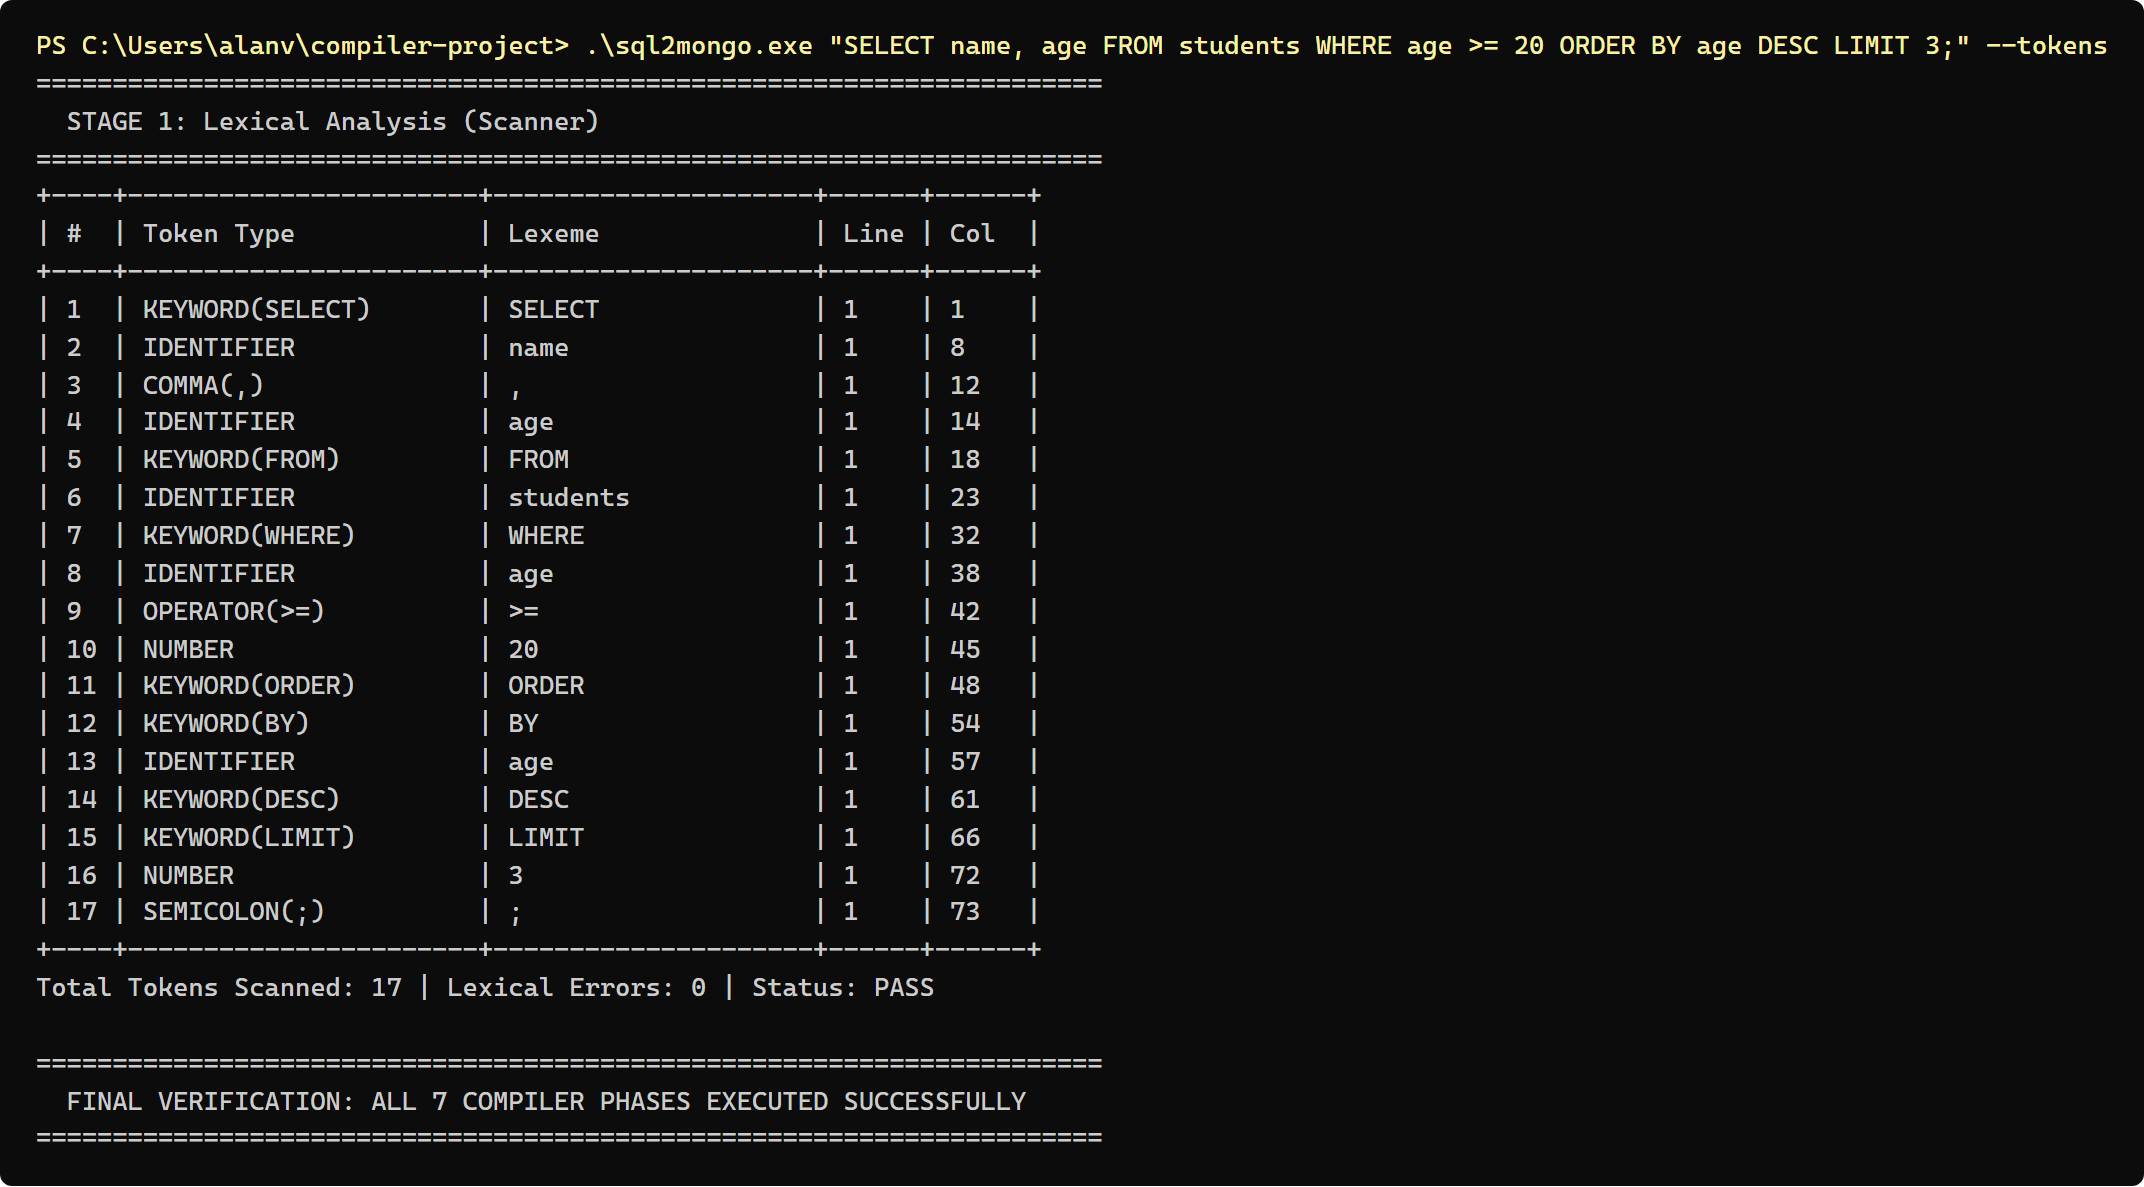
\includegraphics[width=0.82\linewidth]{cli_tokens.png}}
\caption{Token table printed by \code{sql2mongo.exe -{}-tokens} for test case 1}
\label{fig:tokens}
\end{figure}

\section{Syntax Analysis}
The parser (\code{sql\_parser.c}) is a hand-written recursive-descent (LL(1)) parser: one function per non-terminal, deciding each step from the current token only. The grammar in EBNF is:
\begin{Verbatim}[fontsize=\footnotesize]
query         → select_clause from_clause [where_clause]
                [order_clause] [limit_clause] [";"] EOF
select_clause → "SELECT" ( "*" | IDENT { "," IDENT } )
from_clause   → "FROM" IDENT
where_clause  → "WHERE" or_expr
or_expr       → and_expr { "OR" and_expr }
and_expr      → primary { "AND" primary }
primary       → "(" or_expr ")" | IDENT comp_op literal
comp_op       → "=" | "!=" | "<>" | ">" | ">=" | "<" | "<="
literal       → NUMBER | STRING
order_clause  → "ORDER" "BY" IDENT [ "ASC" | "DESC" ]
limit_clause  → "LIMIT" NUMBER
\end{Verbatim}

Precedence comes from the layering: \code{primary} binds tightest, then \code{AND}, then \code{OR}. The \code{\{ \ldots\ \}} repetitions are written as \code{while} loops that fold operands to the left, so \code{a AND b AND c} becomes \code{(a AND b) AND c}. With the \code{-{}-tree} flag the parser prints the concrete parse tree, which records every rule and terminal matched; the WHERE part of the running example is:
\begin{Verbatim}[fontsize=\footnotesize]
<WhereClause>
 ├── Terminal: 'WHERE'
 └── <ConditionExpression>
      └── <ComparisonExpr>
          ├── <FieldIdentifier: "age">
          ├── <ComparisonOp: ">=">
          └── <IntegerLiteral: 20>
\end{Verbatim}

On a syntax error the parser records the first error only and reports the expected construct, for example:
\begin{Verbatim}[fontsize=\footnotesize]
Syntax error at [Line 1, Col 23]: Expected collection/table name identifier,
but found 'WHERE' (KEYWORD(WHERE))
\end{Verbatim}

\section{Abstract Syntax Tree}
The AST (\code{sql\_ast.h}) drops punctuation and keeps meaning. The root \code{ASTQuery} holds the collection name, the projection list (or a wildcard flag), an optional \code{WHERE} tree, and the \code{ORDER BY} and \code{LIMIT} settings. The \code{WHERE} tree is built from \code{ASTFilter} nodes of two kinds:
\begin{itemize}
  \item \textbf{Binary node:} a field, a comparison operator and a typed literal (\code{INT}, \code{FLOAT} or \code{STRING}).
  \item \textbf{Logical node:} \code{AND} or \code{OR} with left and right children.
\end{itemize}
Filter nodes are allocated on the heap and freed recursively by \code{ast\_free} after compilation. Figure~\ref{fig:ast} shows the AST for a query with a parenthesised \code{OR} inside an \code{AND}: the \code{OR} node is the left child of the \code{AND} node, exactly as the grammar's precedence requires.
\begin{figure}[H]
\centering
\fbox{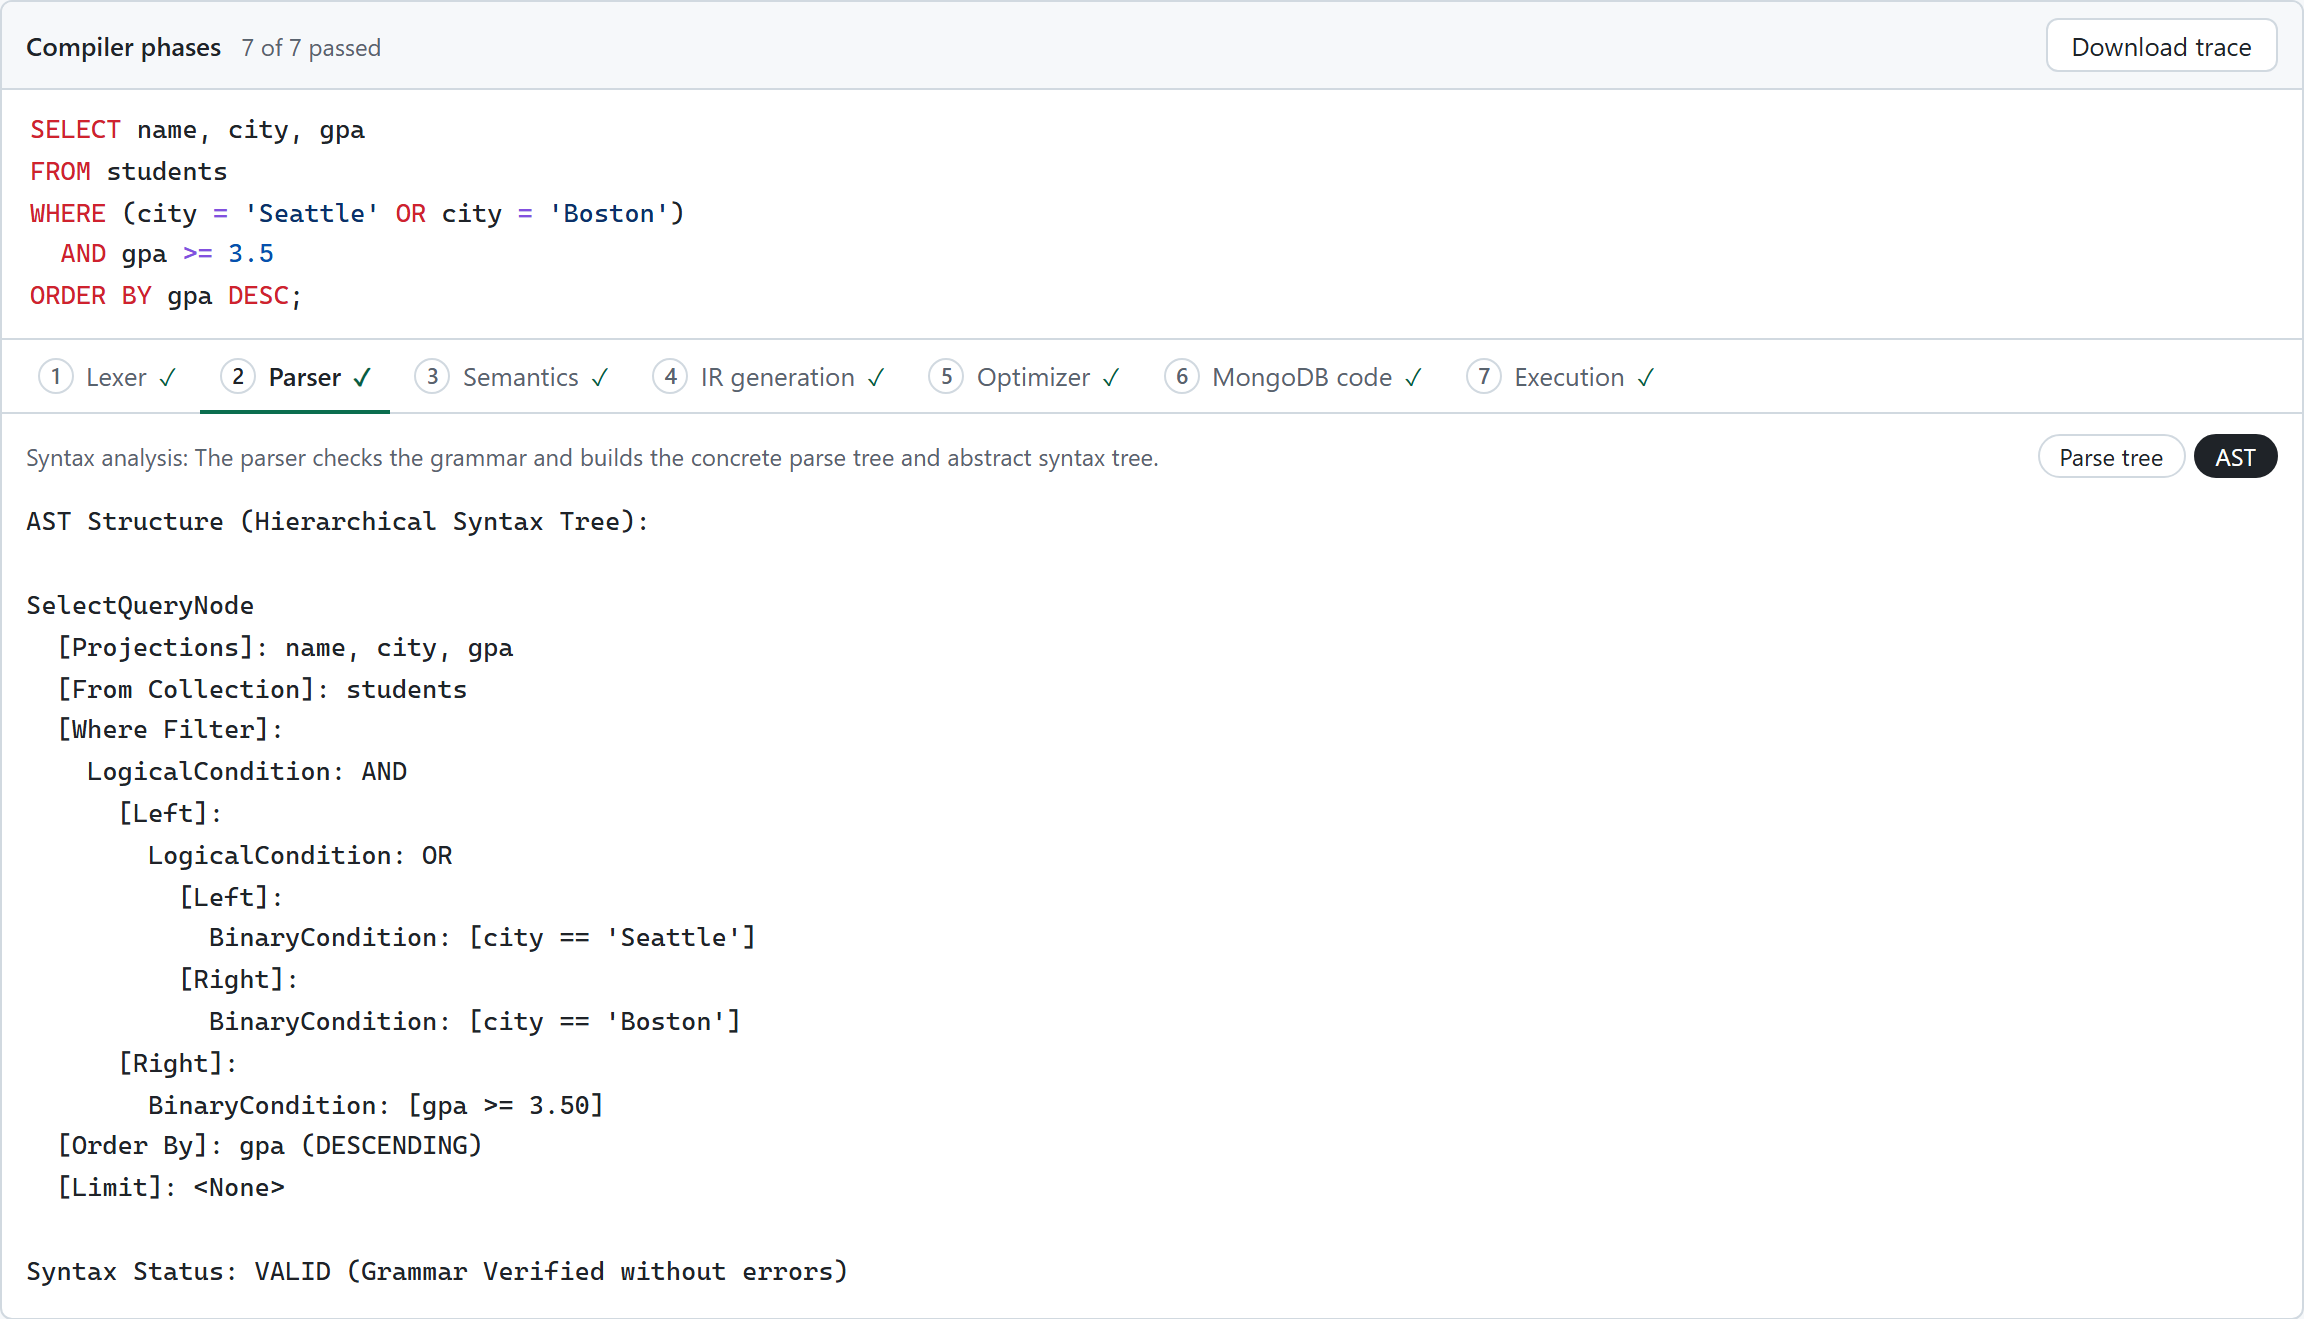
\includegraphics[width=0.82\linewidth]{dash_ast.png}}
\caption{AST for a nested \code{AND}/\code{OR} query, shown on the Compiler phases page}
\label{fig:ast}
\end{figure}

\section{Symbol Table and Semantic Analysis}
The schema catalog (\code{schema\_table.c}) is the symbol table. Each entry is a field symbol scoped to its collection, with a data type and storage width. It holds 2 collections and 10 symbols.
\begin{table}[H]
\centering\small
\begin{tabular}{|l|l|l|l|}
\hline
\textbf{Collection} & \textbf{Field} & \textbf{Type} & \textbf{Width} \\ \hline
students & name, city, status & STRING & 64 B \\ \hline
students & age & INT & 4 B \\ \hline
students & gpa & FLOAT & 8 B \\ \hline
employees & name, department, role & STRING & 64 B \\ \hline
employees & experience & INT & 4 B \\ \hline
employees & salary & FLOAT & 8 B \\ \hline
\end{tabular}
\caption{Symbol table (schema catalog)}
\end{table}

Lookups are case-insensitive. The semantic analyser walks the AST and applies four checks in order, stopping at the first failure:
\begin{enumerate}
  \item The collection in \code{FROM} exists.
  \item Every column in \code{SELECT} exists in that collection.
  \item Every field in \code{WHERE} exists, and its type matches the literal: numeric fields take number literals, string fields take string literals.
  \item The \code{ORDER BY} field exists.
\end{enumerate}
For example, \code{WHERE age = 'twenty'} fails with \code{Semantic Type Error: Cannot compare numeric field 'age' with string literal 'twenty'}. The symbol table is also used by the execution engine to give each number read from a collection file its declared type.

\section{Intermediate Code Generation}
The IR generator (\code{tac.c}) produces three-address code, then derives quadruples and triples from it. It works in two steps:
\begin{enumerate}
  \item \textbf{Condition code.} A post-order walk of the \code{WHERE} tree gives each comparison a new temporary, then combines child temporaries at each \code{AND} or \code{OR} node.
  \item \textbf{Operator chain.} Relational operators are chained in a fixed order, \code{SCAN} $\rightarrow$ \code{FILTER} $\rightarrow$ \code{SORT} $\rightarrow$ \code{LIMIT} $\rightarrow$ \code{PROJECT}, each consuming the previous temporary. Absent clauses are skipped.
\end{enumerate}
For test case 2 (\code{SELECT name, department, salary FROM employees WHERE salary >= 70000 AND department = 'Engineering' ORDER BY salary DESC}) the output is:
\begin{Verbatim}
(1)  t1 = SCAN(employees)
(2)  t2 = salary >= 70000
(3)  t3 = department == 'Engineering'
(4)  t4 = t2 AND t3
(5)  t5 = FILTER(t1, t4)
(6)  t6 = SORT(t5, salary (DESC))
(7)  t7 = PROJECT(t6, [name,department,salary])
\end{Verbatim}
Quadruples store the result temporary explicitly (Figure~\ref{fig:quads}). Triples drop it, and later instructions refer to an earlier result by its index: instruction 4 becomes \code{AND (2) (3)} and instruction 5 becomes \code{FILTER (1) (4)}.
\begin{figure}[H]
\centering
\fbox{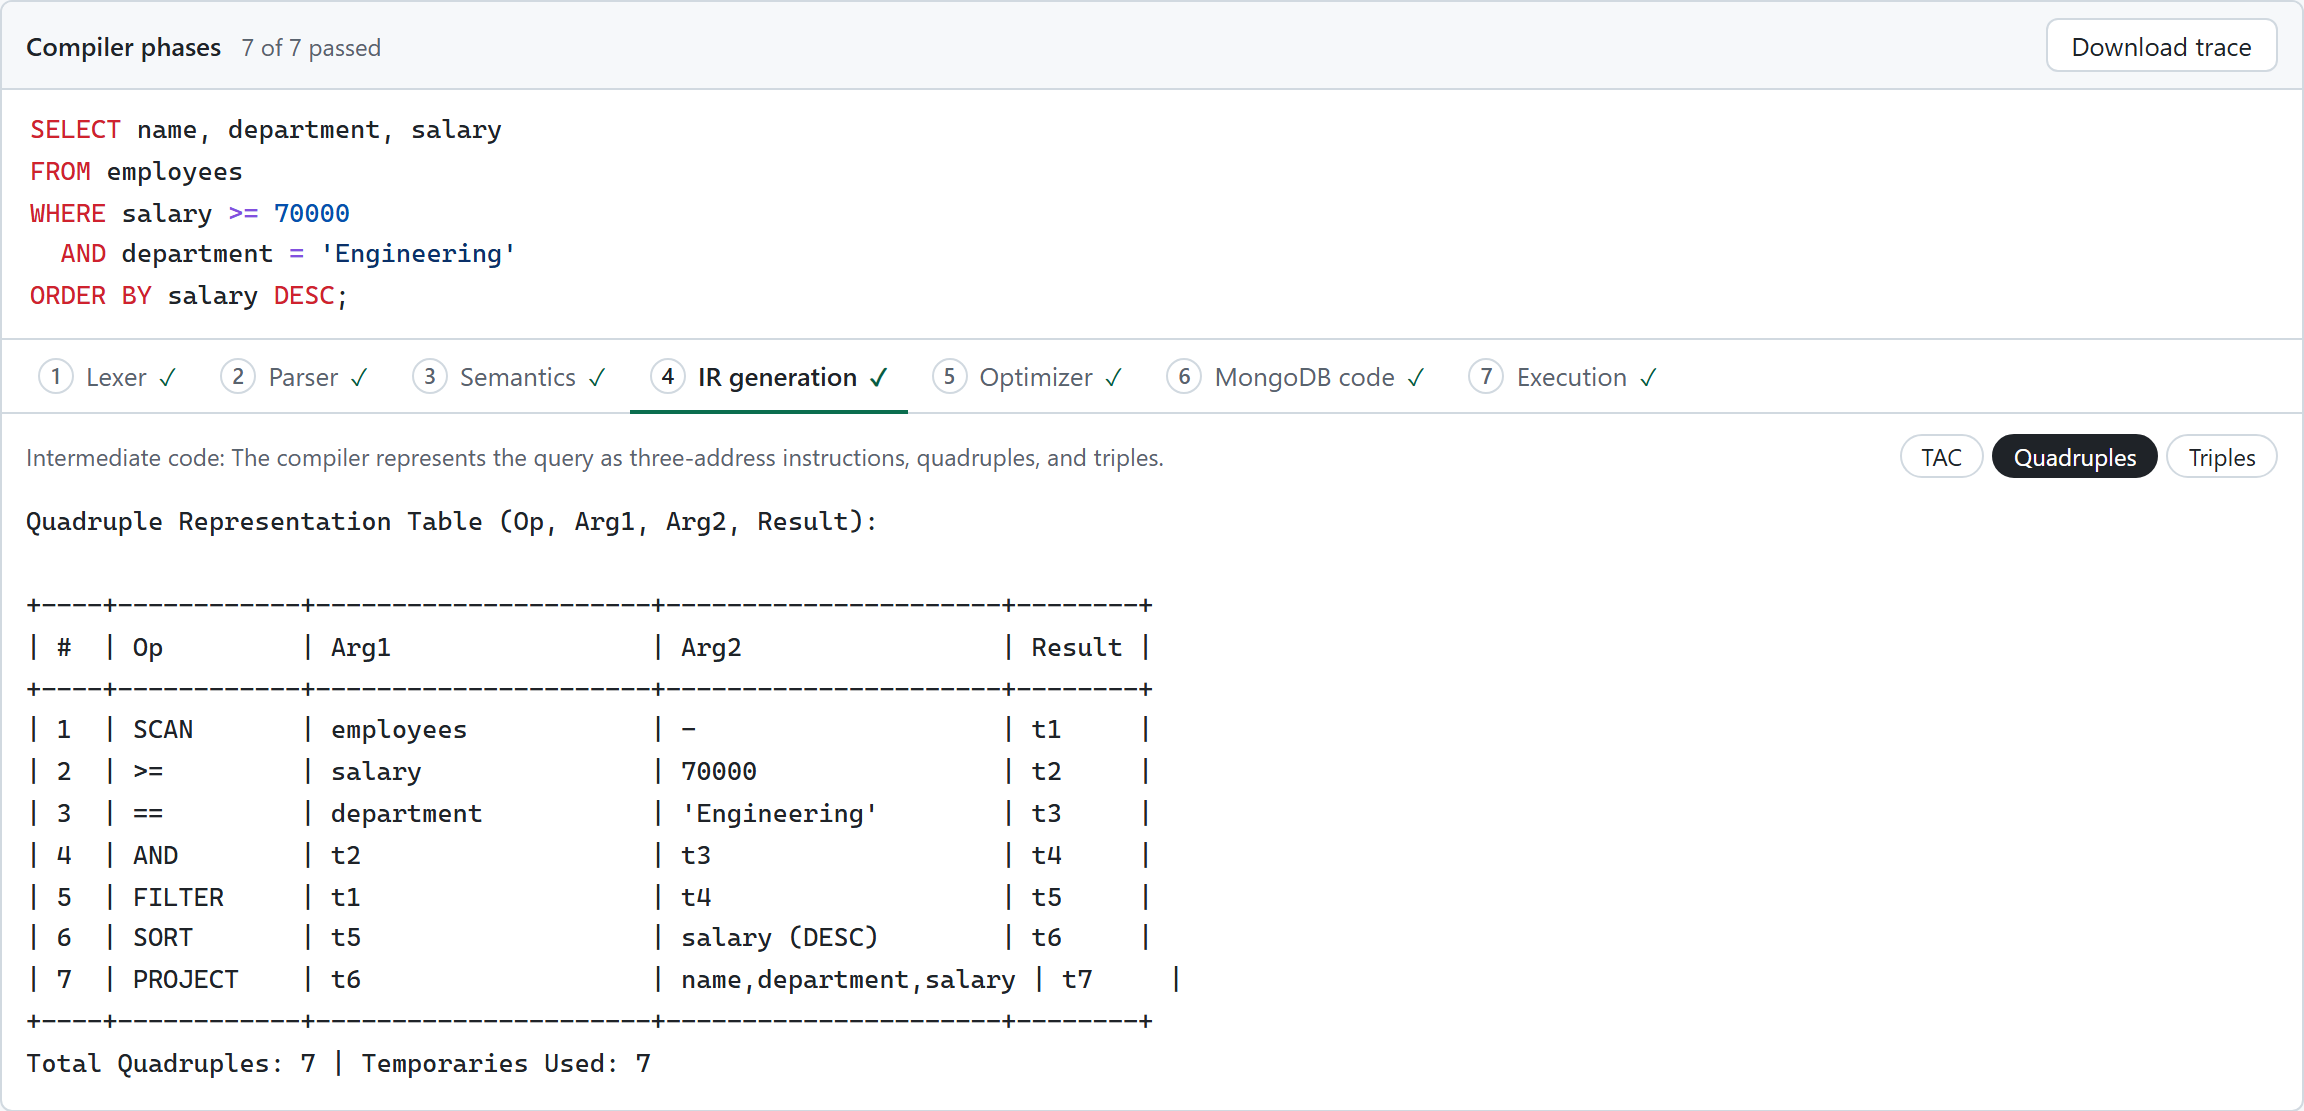
\includegraphics[width=0.82\linewidth]{dash_quads.png}}
\caption{Quadruples for test case 2 on the Compiler phases page}
\label{fig:quads}
\end{figure}

\section{Code Optimization}
The optimizer (\code{optimizer.c}) runs after IR generation and reports which optimizations apply to the query. Two are built into the shape of the IR and of the generated pipeline:
\begin{itemize}
  \item \textbf{Predicate pushdown.} \code{FILTER} always comes straight after \code{SCAN}, so \code{\$match} is always the first pipeline stage. Documents are discarded before the $O(N \log N)$ sort instead of after it.
  \item \textbf{Projection pruning.} A \code{\$project} stage is emitted only when named columns are requested, and it is placed last, as MongoDB's optimization guide recommends \cite{mongo-opt}. For \code{SELECT *} the stage is omitted altogether because it would keep every field.
\end{itemize}
Literal types (\code{INT}, \code{FLOAT}, \code{STRING}) are resolved and checked at compile time, so no type conversion is needed at run time. The grammar has no arithmetic expressions yet, so constant folding currently has nothing to fold; the folding and dead-stage lines of the report are printed for every query.
\begin{Verbatim}[fontsize=\scriptsize]
1. [Predicate Pushdown]       : ENABLED & APPLIED (Filter executed before sort/projection)
2. [Projection Column Pruning]: APPLIED (2 attributes selected)
3. [Compile-Time Folding]     : APPLIED (Static type and literal resolution)
4. [Dead Stage Elimination]   : 0 redundant stages detected
\end{Verbatim}

\section{Target Code Generation}
The code generator (\code{mongo\_codegen.c}) walks the AST and emits a \code{db.<collection>.\allowbreak aggregate([...])} call. Stages appear in the order \code{\$match}, \code{\$sort}, \code{\$limit}, \code{\$project}, and only for clauses present in the query.

Filters are emitted recursively. A comparison becomes \code{\{ field: value \}} for equality or \code{\{ field: \{ \$op: value \} \}} otherwise. A logical node becomes \code{\{ \$and: [left, right] \}} or \code{\{ \$or: [left, right] \}}. Because the AST already encodes precedence, nested conditions come out correctly:
\begin{lstlisting}
SELECT name FROM students
WHERE (age > 19 AND gpa >= 3.5) OR status = 'Graduated'
ORDER BY gpa DESC;
\end{lstlisting}
\begin{lstlisting}
db.students.aggregate([
  { "$match": { "$or": [
      { "$and": [ { "age": { "$gt": 19 } }, { "gpa": { "$gte": 3.50 } } ] },
      { "status": "Graduated" }
  ] } },
  { "$sort": { "gpa": -1 } },
  { "$project": { "_id": 0, "name": 1 } }
]);
\end{lstlisting}

\section{Interpretation and Execution}
The execution engine (\code{engine.c}) is a tree-walking interpreter over the AST. It reads \code{data/<collection>.json} (Section~\ref{sec:jsonreader}), evaluates the \code{WHERE} tree recursively for each document, sorts the matches with \code{qsort} and a field comparator, applies the limit and prints the projected fields as JSON. The query above returns Diana Prince (GPA 3.95), Alice Walker (3.85) and Evan Wright (Graduated, 3.10), which is the correct answer for the data in Appendix~\ref{sec:data}.

\section{Error Detection and Recovery}
Errors are caught in the earliest phase that can see them. The compiler uses a stop-at-first-error strategy: it reports the fault with its position and halts with a phase-specific exit code.
\begin{table}[H]
\centering\footnotesize
\setlength{\tabcolsep}{4pt}
\begin{tabularx}{\linewidth}{|P{1.5cm}|P{2.1cm}|P{3.4cm}|L|c|}
\hline
\textbf{Phase} & \textbf{Error} & \textbf{Example input} & \textbf{Message} & \textbf{Exit} \\ \hline
Lexical & Unknown character & \code{WHERE age @ 20} & \code{Lexical error at [Line 1, Col 42]: Unrecognized or malformed token '@'} & 1 \\ \hline
Lexical & Unterminated string & \code{WHERE city = 'Seattle;} & \code{Lexical error at [Line 1, Col 40]: \ldots\ malformed token 'Seattle;'} & 1 \\ \hline
Syntax & Missing table name & \code{FROM WHERE age >= 20} & \code{Expected collection/table name identifier, but found 'WHERE'} & 1 \\ \hline
Syntax & Unbalanced parenthesis & \code{WHERE (age > 19;} & \code{Expected closing parenthesis ')', but found ';'} & 1 \\ \hline
Semantic & Unknown collection & \code{FROM teachers} & \code{Collection 'teachers' does not exist in schema catalog} & 2 \\ \hline
Semantic & Unknown column & \code{SELECT name, nonexistent\_column} & \code{Column 'nonexistent\_column' in SELECT clause is not defined} & 2 \\ \hline
Semantic & Type mismatch & \code{WHERE city = 25} & \code{Cannot compare string field 'city' with numeric literal} & 2 \\ \hline
Execution & Missing file & \code{FROM employees}, file absent & \code{Cannot open collection file 'data/employees.json'} & 3 \\ \hline
Execution & Invalid JSON & trailing comma in a document & \code{Invalid JSON in 'data/students.json': expected '"' but found '\}'} & 3 \\ \hline
\end{tabularx}
\caption{Error detection by phase}
\end{table}
Figure~\ref{fig:clierrors} shows three of these diagnostics and the exit code of each run.
\begin{figure}[H]
\centering
\fbox{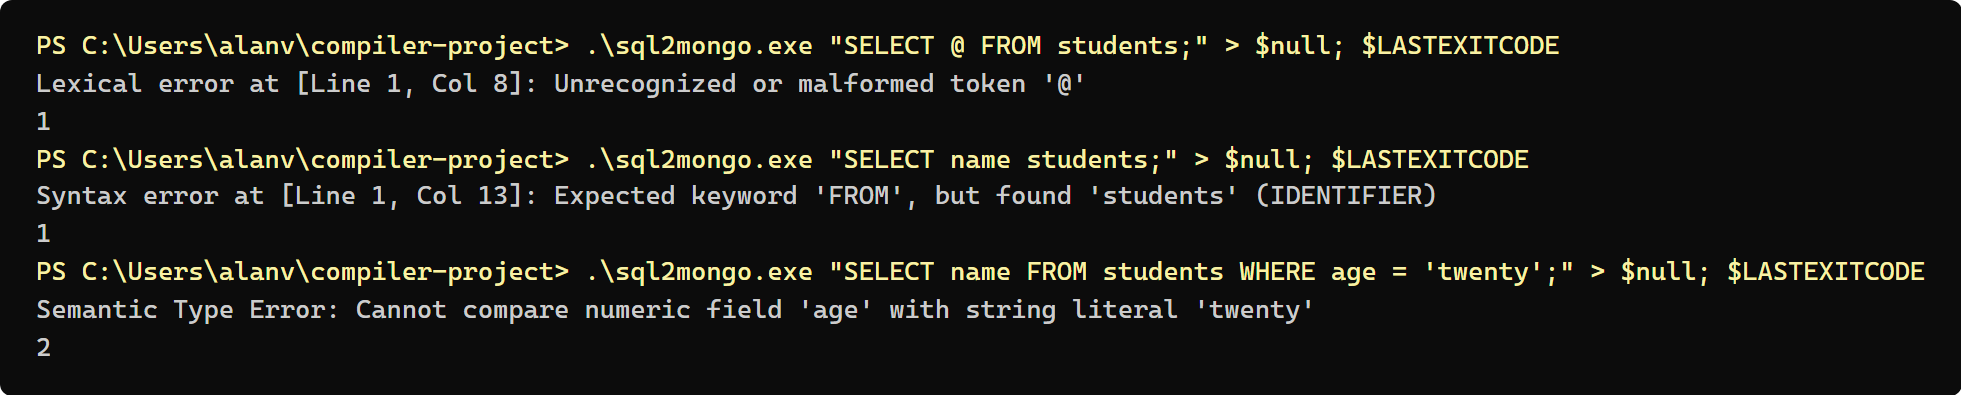
\includegraphics[width=0.92\linewidth]{cli_errors.png}}
\caption{Lexical, syntax and semantic diagnostics with exit codes 1, 1 and 2}
\label{fig:clierrors}
\end{figure}

% =====================================================================
\chapter{Implementation}
% =====================================================================
SQL2Mongo is 2,456 lines of C in ten modules, using only the C standard library. It builds with GCC under \code{-Wall -Wextra} with no warnings. The dashboard adds about 740 lines of JavaScript, HTML and CSS with no third-party packages.

\section{Languages and Tools}
\begin{table}[H]
\centering\small
\begin{tabular}{|l|l|}
\hline
\textbf{Item} & \textbf{Choice} \\ \hline
Compiler language & C, built with \code{-std=c11} \\ \hline
C compiler & GCC 6.3.0 (MinGW) on Windows 11 \\ \hline
C libraries & Standard library only (\code{stdio}, \code{stdlib}, \code{string}, \code{ctype}, \code{stdbool}) \\ \hline
Dashboard & Node.js 20 or newer, built-in modules only; HTML, CSS and JavaScript \\ \hline
Tests & Node.js built-in test runner (\code{node -{}-test}) \\ \hline
Editor and version control & Visual Studio Code, Git \\ \hline
\end{tabular}
\caption{Implementation tools}
\end{table}

\section{Modules}\label{sec:modules}
\begin{table}[H]
\centering\footnotesize
\setlength{\tabcolsep}{4pt}
\begin{tabularx}{\linewidth}{|P{2.3cm}|r|L|P{4.6cm}|}
\hline
\textbf{Module} & \textbf{Lines} & \textbf{Responsibility} & \textbf{Key functions} \\ \hline
\code{sql\_lexer} & 372 & Scanner, token types, token table & \code{lexer\_next\_token}, \code{check\_keyword}, \code{lexer\_print\_all} \\ \hline
\code{sql\_parser} & 395 & Recursive-descent parser, parse-tree printer & \code{parser\_parse}, \code{parse\_or\_expr}, \code{parse\_and\_expr}, \code{parse\_primary\_filter} \\ \hline
\code{sql\_ast} & 223 & AST node types, constructors, printer, cleanup & \code{ast\_create\_binary\_filter}, \code{ast\_create\_logical\_filter}, \code{ast\_free} \\ \hline
\code{schema\_table} & 236 & Symbol table and semantic checks & \code{schema\_init}, \code{schema\_get\_field\_type}, \code{schema\_validate\_query} \\ \hline
\code{tac} & 257 & Three-address code, quadruples, triples & \code{tac\_generate}, \code{quads\_print}, \code{triples\_print} \\ \hline
\code{optimizer} & 59 & Optimization pass and report & \code{optimizer\_run}, \code{optimizer\_print\_report} \\ \hline
\code{query\_plan} & 129 & Relational query plan with cost estimates & \code{plan\_generate}, \code{plan\_print} \\ \hline
\code{mongo\_codegen} & 137 & MQL aggregation-pipeline generator & \code{mongo\_codegen\_pipeline}, \code{emit\_filter\_json} \\ \hline
\code{engine} & 381 & JSON collection reader and query interpreter & \code{load\_collection}, \code{json\_read\_document}, \code{eval\_filter}, \code{engine\_execute\_query} \\ \hline
\code{main} & 267 & Command-line driver that runs the phases in order & \code{main}, \code{read\_entire\_file}, \code{resolve\_data\_dir} \\ \hline
\textbf{Total} & \textbf{2,456} & & \\ \hline
\end{tabularx}
\caption{Source modules (lines counted over the \code{.c} and \code{.h} files)}
\end{table}

\section{Key Algorithms}
\begin{itemize}
  \item \textbf{Scanning:} a character-class switch with one-character lookahead and maximal munch; keywords found by upper-casing the identifier and comparing it with the keyword list. Linear in input length.
  \item \textbf{Parsing:} LL(1) recursive descent with one token of lookahead; left-associative operator chains built by loops. Linear in the number of tokens.
  \item \textbf{Semantic analysis:} recursive AST walk with linear symbol lookup in the catalog (10 symbols).
  \item \textbf{IR generation:} post-order traversal of the filter tree; a counter supplies fresh temporaries \code{t1, t2, \ldots}. Triples are derived by replacing each temporary with the index of the quadruple that produced it.
  \item \textbf{Code generation:} recursive emission of nested JSON for \code{\$and} and \code{\$or}.
  \item \textbf{Execution:} one pass over the collection file to read it, per-document recursive evaluation of the filter tree, \code{qsort} for \code{ORDER BY}, then limit and projection.
\end{itemize}

\section{Reading Collection Files}\label{sec:jsonreader}
The engine contains a small recursive-descent reader for the collection format: an array of flat objects whose values are strings or numbers. It is a second, much smaller parser in the same style as the SQL parser, with one function per construct (\code{json\_read\_string}, \code{json\_read\_document}, \code{load\_collection}).
\begin{itemize}
  \item \textbf{Locating the file.} The collection name is lower-cased and the file \code{data/<name>.json} is opened. \code{main.c} looks for \code{data/} in the working directory first and then next to the executable, so the compiler works from any folder.
  \item \textbf{Typing values.} A string becomes \code{TYPE\_STRING}. A number takes the type declared in the symbol table, so \code{95000} and \code{95000.0} are both read as \code{FLOAT} for \code{salary}. A number in an undeclared field is \code{INT}, or \code{FLOAT} if it has a decimal point or exponent. \code{true}, \code{false} and \code{null} are skipped.
  \item \textbf{Strings.} The escapes \code{\textbackslash"}, \code{\textbackslash\textbackslash}, \code{\textbackslash/}, \code{\textbackslash n}, \code{\textbackslash t} and \code{\textbackslash r} are decoded when reading and encoded again when printing results, so the output is always valid JSON.
  \item \textbf{Errors.} A missing file or a syntax error in the file is reported with the file name and what was expected, and the compiler exits with code 3.
\end{itemize}
The file is read each time a query runs, so editing a collection changes the next result without rebuilding.

\section{Web Dashboard}
The dashboard is a Node.js server (\code{server.mjs}), a bridge to the compiler (\code{compiler.mjs}) and a single web page with three views.
\begin{itemize}
  \item \textbf{Running the compiler.} For each query the bridge writes the SQL to its own temporary file, starts \code{sql2mongo.exe} with \code{-{}-all} without a shell, and waits for it to finish.
  \item \textbf{Parsing the output.} The output is split at the \code{STAGE n} banners. Tokens and symbol-table rows are read from their text tables, the pipeline is read from the \code{db.\ldots;} block, and each result document is parsed as JSON. The exit code and diagnostic decide which phase failed.
  \item \textbf{Query page.} SQL editor with syntax highlighting and seven example queries, the generated pipeline, and the result documents as JSON or a table (Figure~\ref{fig:query}).
  \item \textbf{Compiler phases page.} One tab per phase, marked as passed, failed or not reached, with sub-tabs for the parse tree and AST and for TAC, quadruples and triples (Figure~\ref{fig:phases}).
  \item \textbf{Database page.} The documents in each collection file with the field types from the symbol table (Figure~\ref{fig:database}).
\end{itemize}

\section{Limits and Safety}
\begin{table}[H]
\centering\small
\begin{tabularx}{\linewidth}{|P{5.2cm}|P{2.2cm}|L|}
\hline
\textbf{Limit} & \textbf{Value} & \textbf{Behaviour when exceeded} \\ \hline
Documents per collection & 32 & Exit code 3 with a message \\ \hline
Fields per document & 16 & Extra fields are ignored \\ \hline
String value length & 127 characters & The value is truncated \\ \hline
IR instructions & 32 & Further instructions are not generated \\ \hline
Query length (dashboard) & 4,000 characters & Rejected with HTTP 400 \\ \hline
Request body (dashboard) & 16 KB & Rejected with HTTP 413 \\ \hline
Compiler run time (dashboard) & 6 seconds & Process stopped; HTTP 504 \\ \hline
Simultaneous compilations & 4 & Rejected with HTTP 429 \\ \hline
\end{tabularx}
\caption{Limits and their behaviour}
\end{table}
The server listens on \code{127.0.0.1} only, rejects requests from other origins (HTTP 403) and serves only its own four files. The input is always treated as SQL text and never as a file path.

\section{Problems Found and Fixed During Phase 3}
\begin{enumerate}
  \item \textbf{The data files were not used.} The execution engine held its documents in C code and ignored \code{data/*.json}, so editing a file had no effect. The JSON reader of Section~\ref{sec:jsonreader} replaced the built-in records.
  \item \textbf{Result strings were not escaped.} A quotation mark inside a value would have produced invalid JSON output. Strings are now escaped when printed.
  \item \textbf{Execution errors were reported as success.} The result of the execution engine was ignored, so a missing collection still ended with \code{ALL 7 COMPILER PHASES EXECUTED SUCCESSFULLY}. The compiler now stops with exit code 3.
  \item \textbf{The data folder depended on the working directory.} Running the compiler from another folder could not find the collections. \code{resolve\_data\_dir} now also looks next to the executable.
\end{enumerate}

% =====================================================================
\chapter{Testing and Results}
% =====================================================================
\section{Test Strategy}
Tests cover valid, boundary, lexical-error, syntax-error, semantic-error and execution-error inputs. Each case has a known correct exit code and, where it succeeds, a known set of result documents that can be checked by hand against Appendix~\ref{sec:data}. Nine integration tests check the most important cases and the dashboard API automatically. All tests were run on 28 October 2026 with a fresh build of the current source.

\section{How the Tests Are Run}
\begin{table}[H]
\centering\small
\begin{tabularx}{\linewidth}{|P{6.4cm}|L|}
\hline
\textbf{Command} & \textbf{Result} \\ \hline
\code{npm run build:compiler} (in \code{dashboard/}) & Rebuilds \code{sql2mongo.exe} from \code{src/*.c}; no warnings \\ \hline
\code{npm test} (in \code{dashboard/}) & The 9 integration tests of Table~\ref{tab:integration} \\ \hline
\code{sql2mongo.exe "<query>" -{}-all} & Test cases 1--19, compared with the expected exit code and output \\ \hline
Compiler run from a folder whose \code{data/} has a missing or broken file & Test cases 20--21 \\ \hline
\end{tabularx}
\caption{How the tests are run}
\end{table}
\begin{figure}[H]
\centering
\fbox{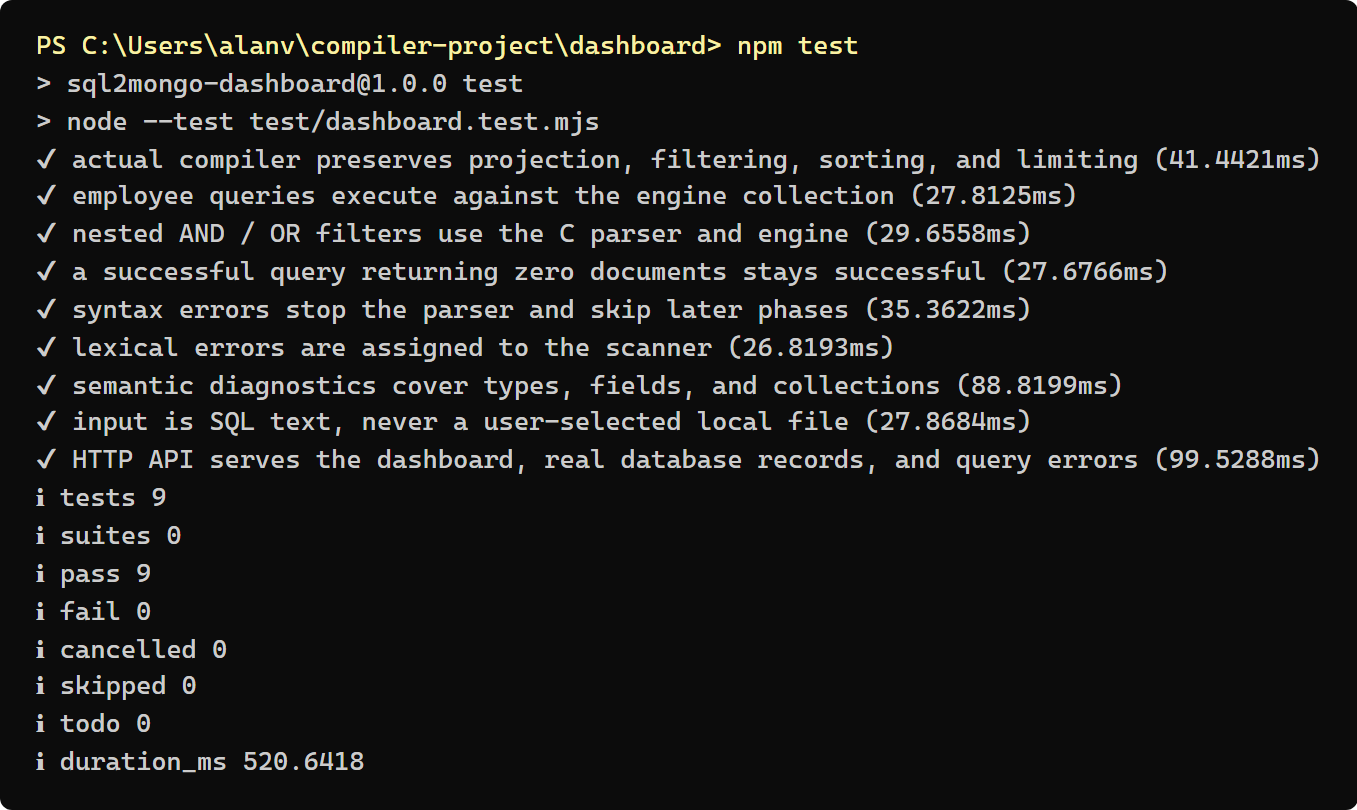
\includegraphics[width=0.62\linewidth]{npm_test.png}}
\caption{Automated test run: 9 of 9 integration tests pass}
\label{fig:npmtest}
\end{figure}

\section{Test Cases and Results}
{\footnotesize
\setlength{\tabcolsep}{3.5pt}
\begin{longtable}{|>{\raggedright\arraybackslash}p{0.45cm}|>{\raggedright\arraybackslash}p{1.75cm}|>{\raggedright\arraybackslash}p{4.9cm}|>{\raggedright\arraybackslash}p{2.4cm}|>{\raggedright\arraybackslash}p{3.2cm}|>{\raggedright\arraybackslash}p{1.1cm}|}
\caption{Test cases and results}\\
\hline
\textbf{\#} & \textbf{Category} & \textbf{Input (query or clause)} & \textbf{Expected} & \textbf{Actual} & \textbf{Status} \\ \hline
\endfirsthead
\hline
\textbf{\#} & \textbf{Category} & \textbf{Input (query or clause)} & \textbf{Expected} & \textbf{Actual} & \textbf{Status} \\ \hline
\endhead
1 & Valid & \code{SELECT name, age FROM students WHERE age >= 20 ORDER BY age DESC LIMIT 3;} & Exit 0; 3 documents, oldest first & Diana (23), Alice (22), Bob (21) & Pass \\ \hline
2 & Valid, \code{AND} & \code{SELECT name, department, salary FROM employees WHERE salary >= 70000 AND department = 'Engineering' ORDER BY salary DESC;} & Exit 0; \code{\$and} filter & Sarah Connor (95000), John Doe (72000) & Pass \\ \hline
3 & Valid, \code{*} and float & \code{SELECT * FROM students WHERE gpa >= 3.85;} & Exit 0; no \code{\$project} stage & 3 full documents; pipeline has \code{\$match} only & Pass \\ \hline
4 & Valid, \code{OR} & \code{SELECT name, city FROM students WHERE city = 'Seattle' OR city = 'Boston' ORDER BY name ASC;} & Exit 0; \code{\$or} filter, sorted by name & Alice, Bob, Charlie & Pass \\ \hline
5 & Complex & \code{WHERE (age > 19 AND gpa >= 3.5) OR status = 'Graduated' ORDER BY gpa DESC} & \code{\$and} nested inside \code{\$or} & Correct nesting; Diana, Alice, Evan & Pass \\ \hline
6 & Boundary & \code{WHERE age > 100} & Exit 0; empty result & 0 documents returned & Pass \\ \hline
7 & Boundary & \code{select NAME, Age from STUDENTS where AGE < 21 limit 1} (mixed case, no \code{;}) & Exit 0; 1 document & Charlie Brown returned; MQL keeps the user's casing & Partial \\ \hline
8 & Boundary & \code{LIMIT 0} & Rejected, or valid MQL & Accepted; emits \code{\$limit: 0} & Partial \\ \hline
9 & Lexical error & \code{WHERE age @ 20} & Exit 1 & Exit 1, unrecognised token \code{'@'} at col 42 & Pass \\ \hline
10 & Lexical error & \code{WHERE city = 'Seattle;} & Exit 1 & Exit 1, unterminated string reported & Pass \\ \hline
11 & Syntax error & \code{SELECT name, age FROM WHERE age >= 20;} & Exit 1 & Exit 1, expected table name, at col 23 & Pass \\ \hline
12 & Syntax error & \code{ORDER age} & Exit 1 & Exit 1, expected \code{BY} after \code{ORDER} & Pass \\ \hline
13 & Syntax error & \code{LIMIT 2 extra;} & Exit 1 & Exit 1, unexpected trailing tokens & Pass \\ \hline
14 & Syntax error & \code{WHERE (age > 19;} & Exit 1 & Exit 1, expected closing parenthesis & Pass \\ \hline
15 & Semantic error & \code{SELECT name, nonexistent\_column FROM students WHERE age = 'twenty';} & Exit 2 & Exit 2, unknown column reported first & Pass \\ \hline
16 & Semantic error & \code{WHERE age = 'twenty'} & Exit 2 & Exit 2, numeric field compared with string & Pass \\ \hline
17 & Semantic error & \code{WHERE city = 25} & Exit 2 & Exit 2, string field compared with number & Pass \\ \hline
18 & Semantic error & \code{FROM teachers} & Exit 2 & Exit 2, collection does not exist & Pass \\ \hline
19 & Semantic error & \code{FROM students ORDER BY salary} & Exit 2 & Exit 2, \code{ORDER BY} field does not exist & Pass \\ \hline
20 & Execution error & \code{SELECT name FROM employees;} with \code{employees.json} absent & Exit 3 & Exit 3, file cannot be opened & Pass \\ \hline
21 & Execution error & \code{SELECT name FROM students;} with a trailing comma in \code{students.json} & Exit 3 & Exit 3, invalid JSON reported with its position & Pass \\ \hline
\end{longtable}
}

\section{Automated Integration Tests}
The integration tests in \code{dashboard/test/dashboard.test.mjs} run the real executable and the real server.
\begin{table}[H]
\centering\footnotesize
\begin{tabularx}{\linewidth}{|P{3.4cm}|L|P{1.0cm}|}
\hline
\textbf{Test} & \textbf{What is checked} & \textbf{Result} \\ \hline
Projection, filter, sort, limit & Exact documents returned; 19 tokens; 10 symbols; stages \code{\$match}, \code{\$sort}, \code{\$limit}, \code{\$project}; all 7 phases complete & Pass \\ \hline
Second collection & Employee query on \code{department} returns the two engineers in salary order & Pass \\ \hline
Nested \code{AND} / \code{OR} & Parenthesised filter returns the right documents and emits \code{\$and} & Pass \\ \hline
Empty result & A valid query matching nothing still succeeds with 0 documents & Pass \\ \hline
Syntax error & Phase 2 fails, phases 3 to 7 are skipped, no pipeline is produced & Pass \\ \hline
Lexical error & The error is assigned to phase 1 and all later phases are skipped & Pass \\ \hline
Semantic errors & Wrong type, unknown field and unknown collection all stop at phase 3 & Pass \\ \hline
Input handling & Input is always SQL, never a file path; empty, oversized and null-byte input rejected & Pass \\ \hline
HTTP API & Pages served; database matches \code{data/students.json}; bad JSON 400, other origin 403, wrong content type 415, source files 404 & Pass \\ \hline
\end{tabularx}
\caption{Automated integration tests (9 of 9 pass in about 0.5 s)}
\label{tab:integration}
\end{table}

\section{Performance Evaluation}
A complete seven-phase run averaged 50.1\,ms for test case 1 and 52.7\,ms for test case 2, over 100 runs each. A run that only prints the help text averaged 30.8\,ms, so process start-up dominates. The compiler phases, reading the collection file and printing the output account for about 20\,ms. Through the dashboard, a query takes roughly 35 to 130\,ms from request to response.

Memory use is fixed: every structure has a static size, and the largest, the engine's two arrays of 32 documents, take about 213\,KB.

\section{Output Evidence}
Figure~\ref{fig:clirun} shows the generated pipeline and the execution results for test case 1 from the command line. The remaining figures show the dashboard: a successful query (Figure~\ref{fig:query}), a query stopped by a semantic error (Figure~\ref{fig:phases}), and the stored collection (Figure~\ref{fig:database}).
\begin{figure}[H]
\centering
\fbox{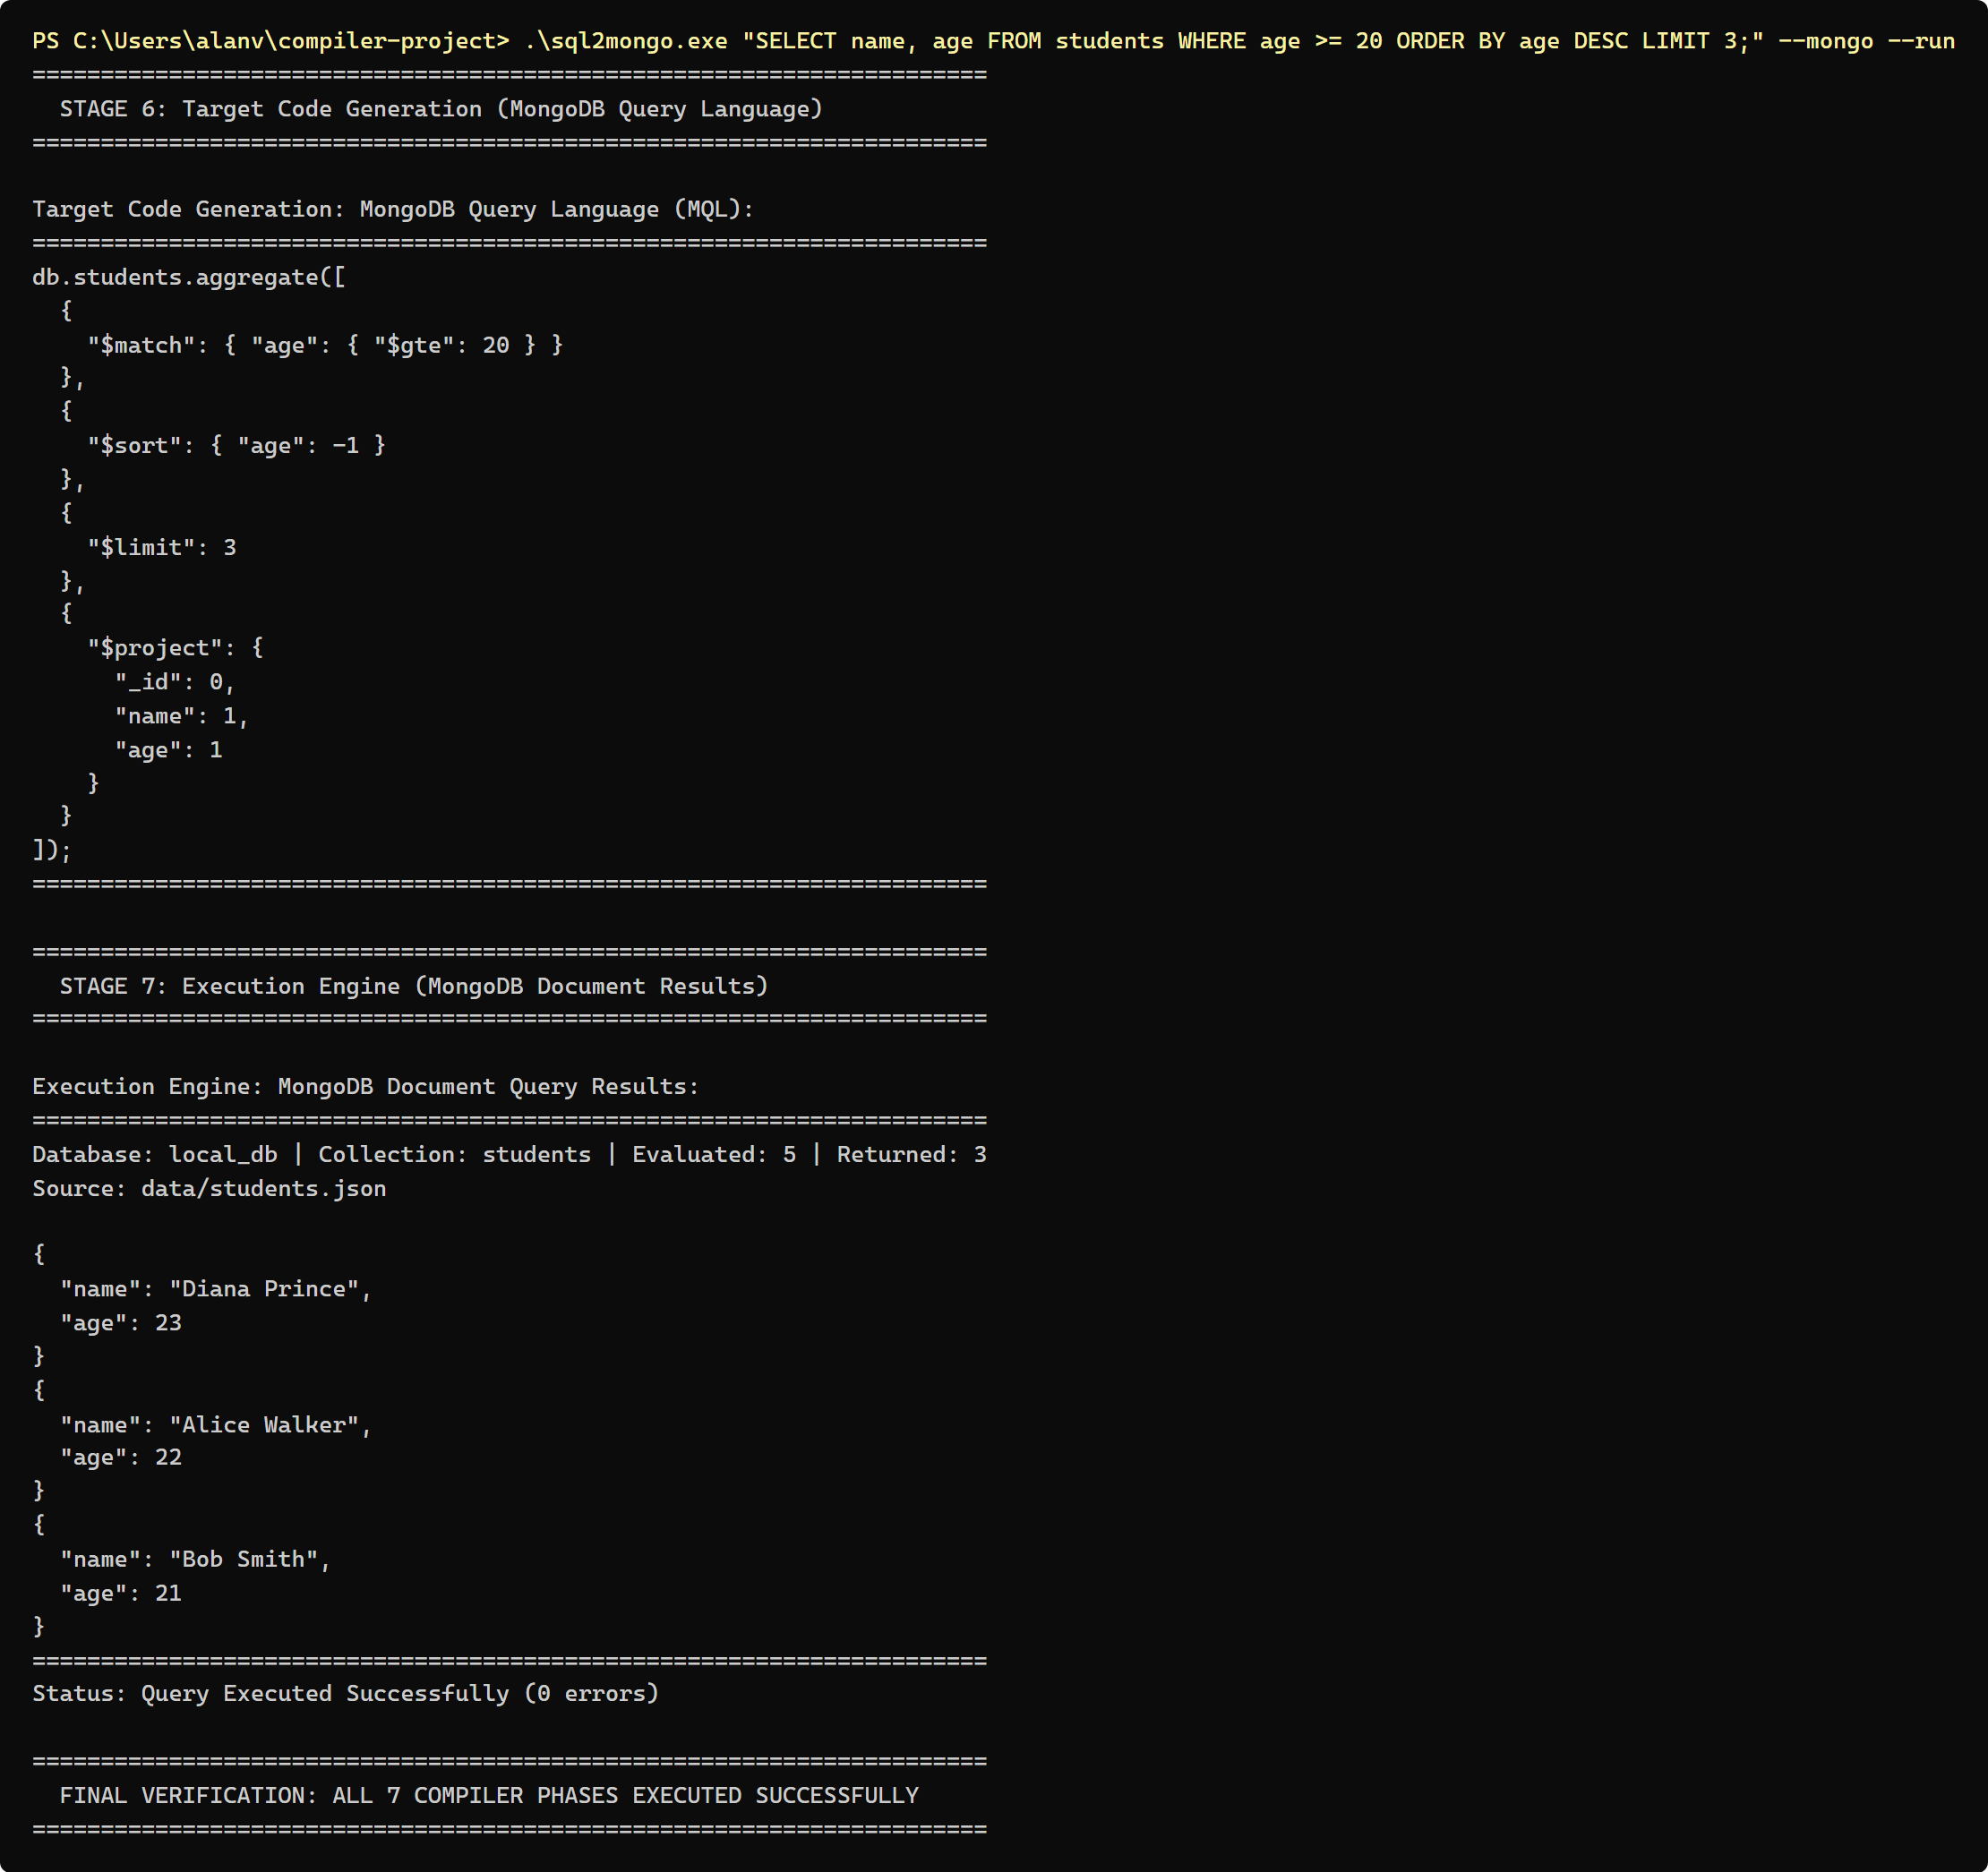
\includegraphics[width=0.7\linewidth,height=0.5\textheight,keepaspectratio]{cli_run.png}}
\caption{Test case 1 with \code{-{}-mongo -{}-run}: the pipeline, then three documents read from \code{data/students.json}}
\label{fig:clirun}
\end{figure}
\begin{figure}[H]
\centering
\fbox{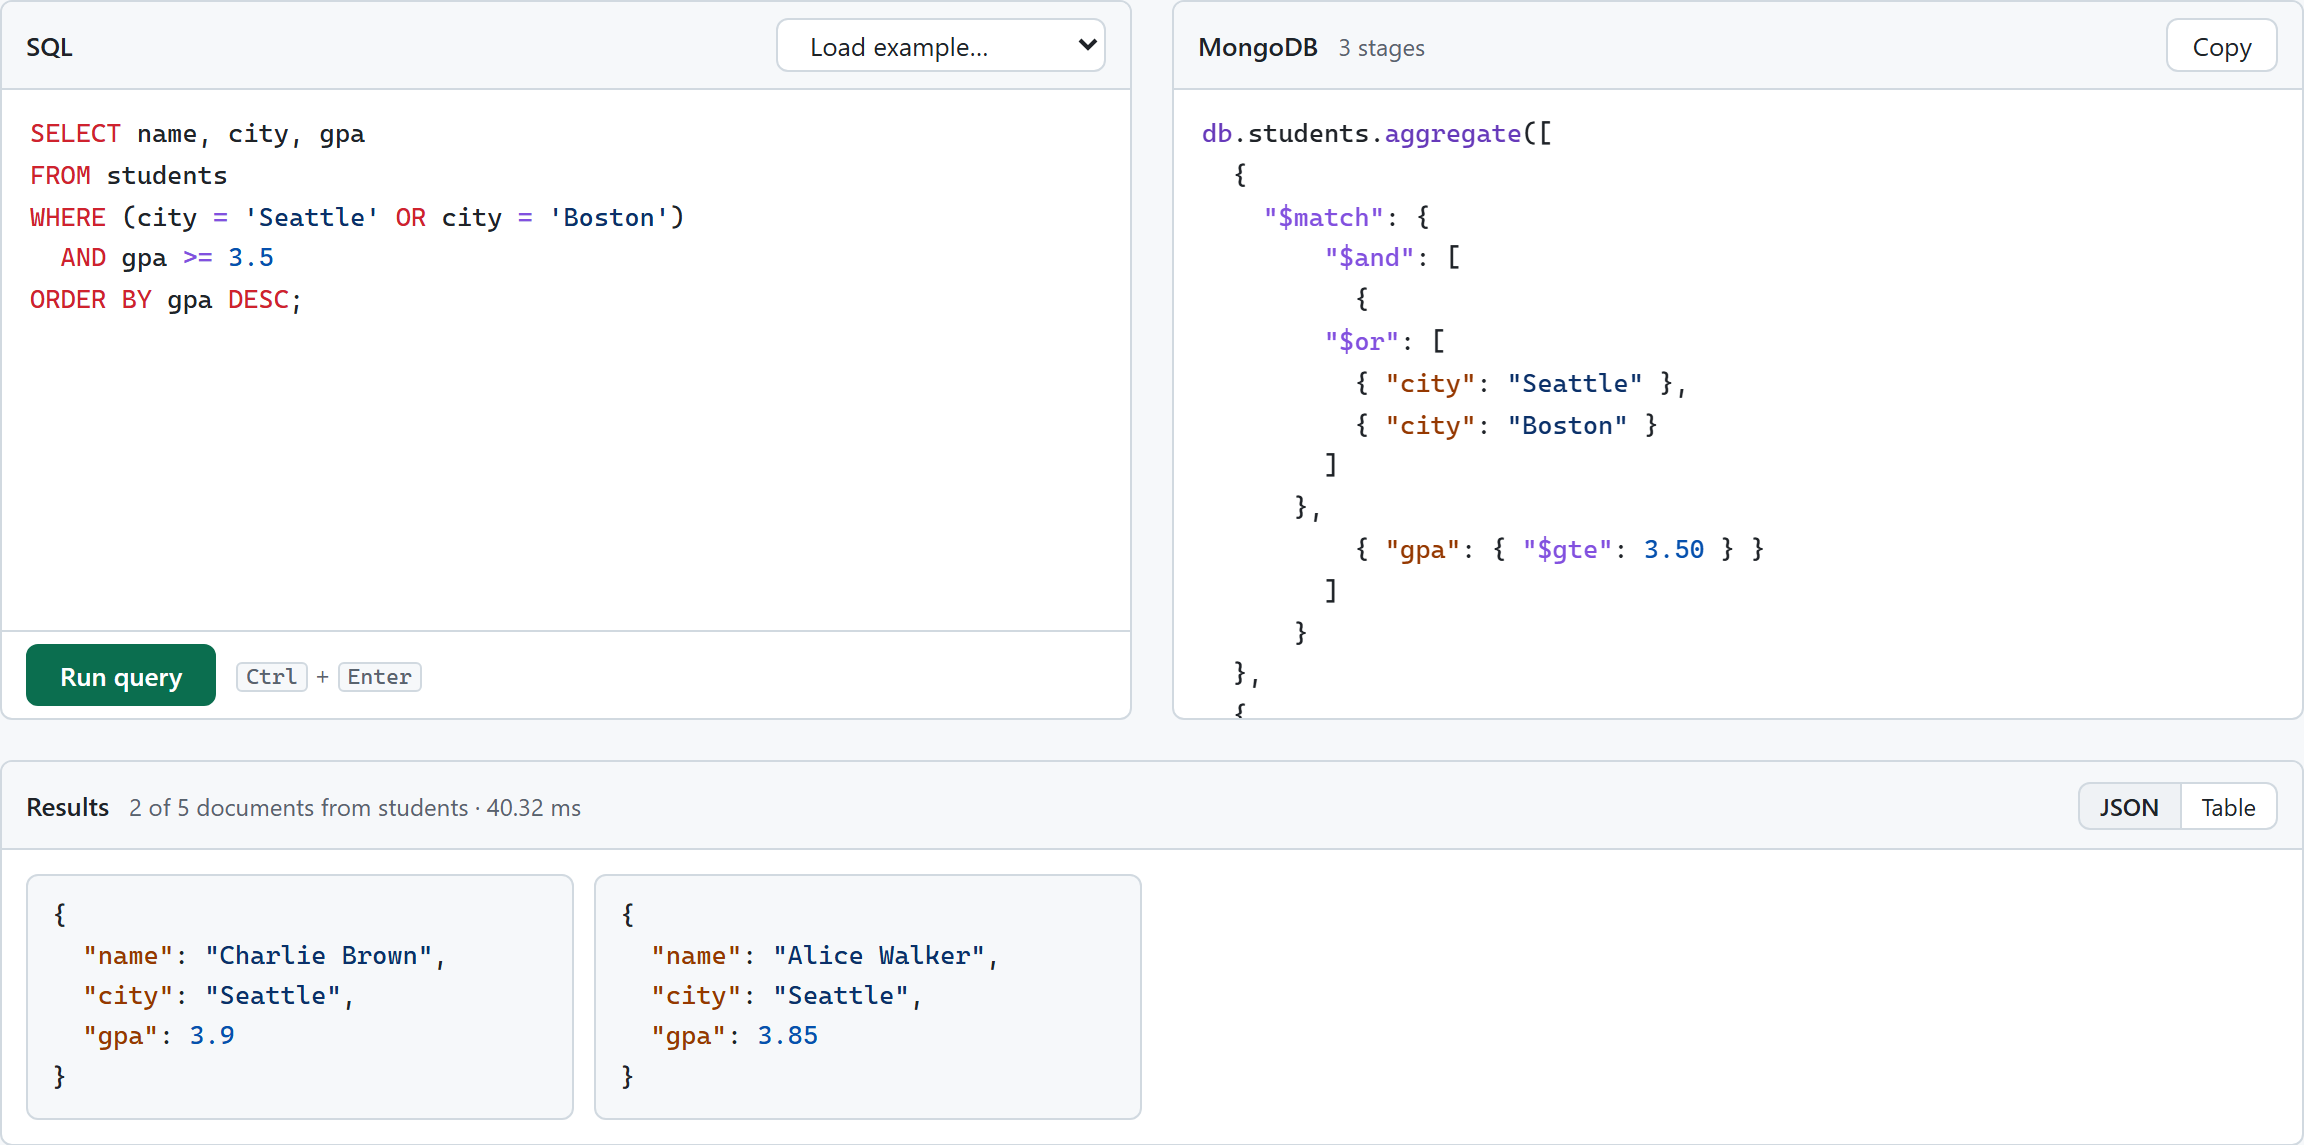
\includegraphics[width=0.86\linewidth]{dash_query_andor.png}}
\caption{Query page: SQL with nested \code{AND}/\code{OR}, the generated pipeline and the two result documents}
\label{fig:query}
\end{figure}
\begin{figure}[H]
\centering
\fbox{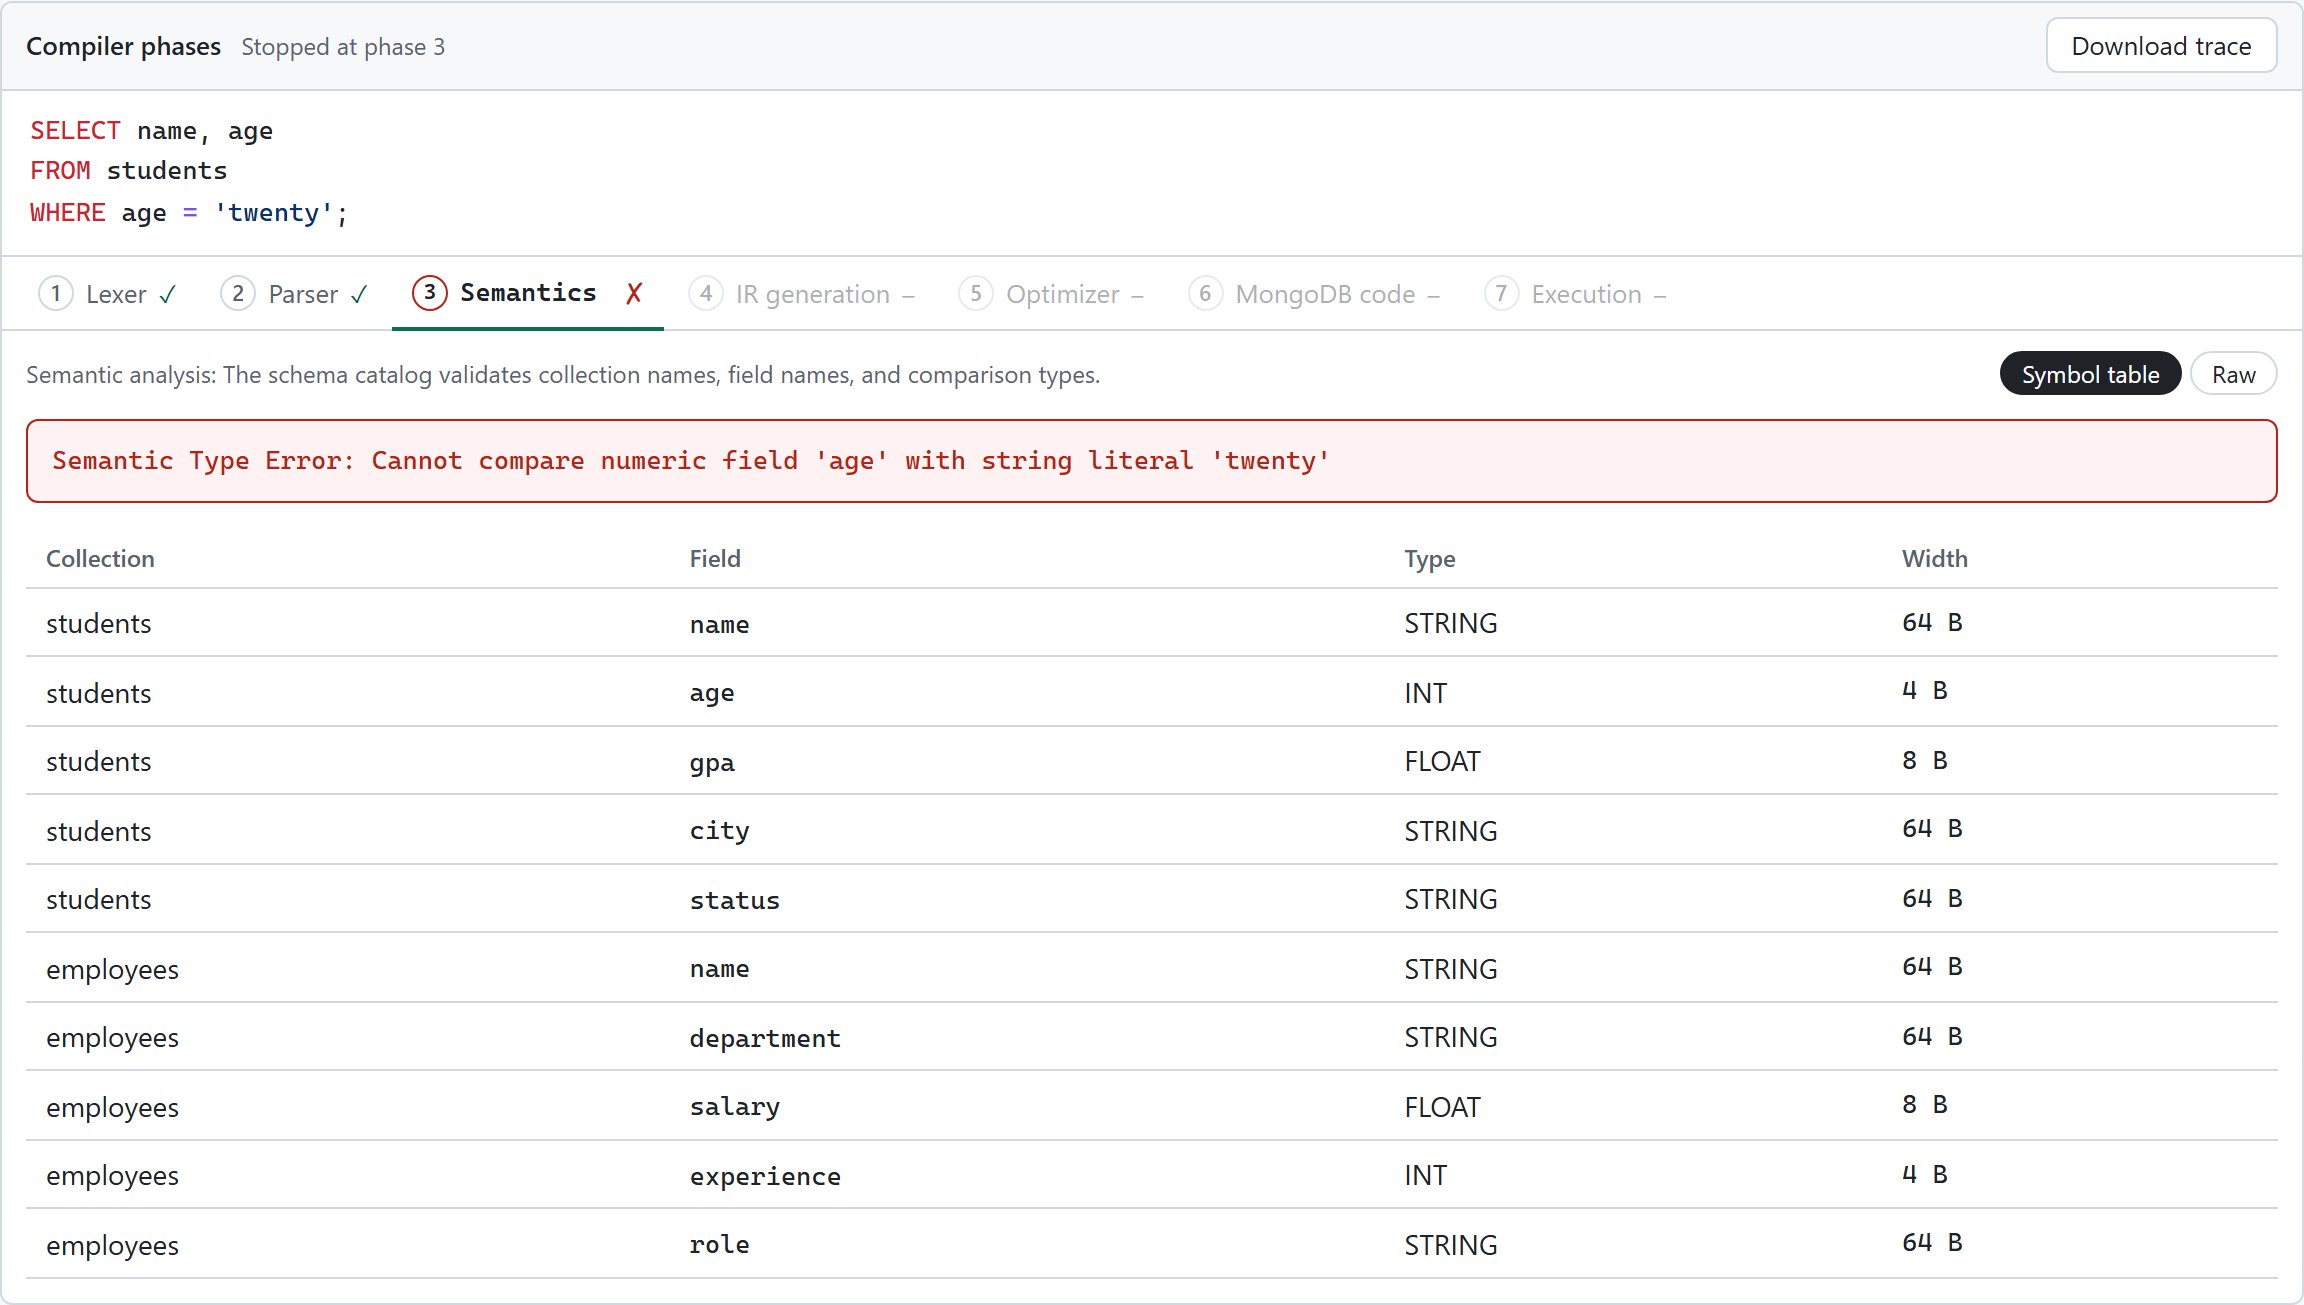
\includegraphics[width=0.86\linewidth]{dash_error_phases.png}}
\caption{Compiler phases page for \code{WHERE age = \textquotesingle twenty\textquotesingle}: phase 3 fails with the type error and phases 4 to 7 are not reached}
\label{fig:phases}
\end{figure}
\begin{figure}[H]
\centering
\fbox{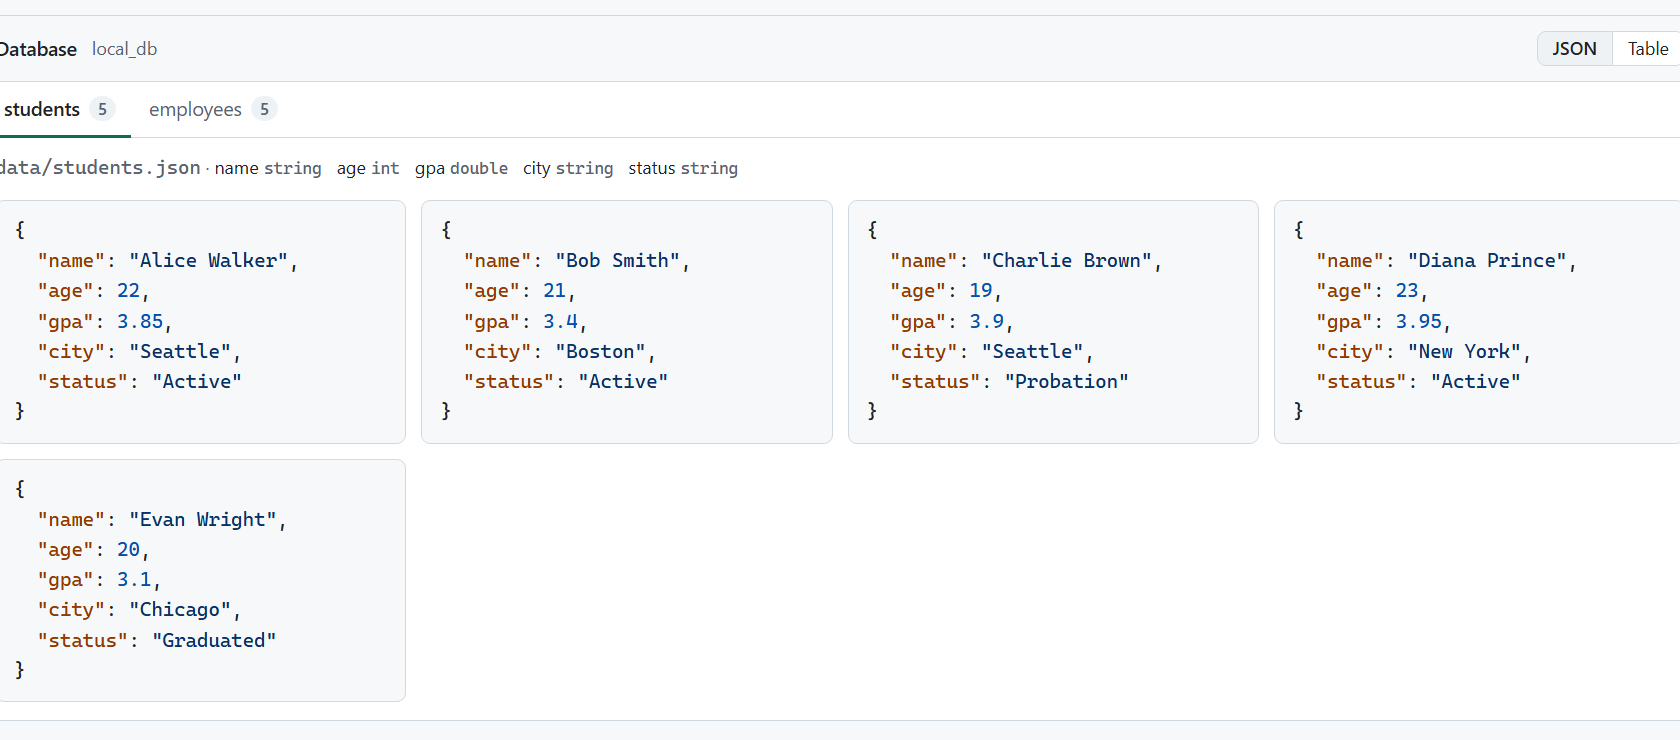
\includegraphics[width=0.86\linewidth]{database_json.png}}
\caption{Database page: the \code{students} collection as stored in \code{data/students.json}}
\label{fig:database}
\end{figure}

\section{Findings}\label{sec:findings}
\begin{itemize}
  \item \textbf{Case 7:} keywords and schema lookups are case-insensitive, but the generator copies identifiers as typed. MongoDB is case-sensitive, so \code{db.STUDENTS} and \code{"AGE"} would match nothing on a real server. Identifiers should be normalised to their catalog spelling.
  \item \textbf{Case 8:} MongoDB's \code{\$limit} stage takes a positive integer \cite{mongo-limit}, so \code{LIMIT 0} should be rejected during semantic analysis.
\end{itemize}

\section{Summary of Results}
Of 21 test queries, 19 behave exactly as expected and 2 are partial (cases 7 and 8); both partial cases run correctly in the engine but produce MQL that a real MongoDB server would treat differently. All 9 automated integration tests pass, and the compiler builds without warnings.

% =====================================================================
\chapter{Conclusion}
% =====================================================================
SQL2Mongo meets all nine objectives: it compiles a useful subset of SQL into valid MongoDB aggregation pipelines through seven hand-built phases, catches lexical, syntax and semantic errors before any code is generated, and checks each translation by running it on collections stored in the same JSON format MongoDB exports.

The project started from a practical problem I ran into during my internship: knowing SQL well, but having to write MongoDB queries. SQL2Mongo removes the need to translate each query by hand. Its phase-by-phase output, now also shown in the web dashboard, explains how each SQL clause maps to its MongoDB form, so it doubles as a learning aid for anyone making the same switch.

The project shows that the classic compiler pipeline carries over directly to query translation. Lexing, recursive-descent parsing, symbol tables, three-address code and code generation each have a clear job, and the AST holds them together. The same parsing technique was reused for the collection files. The visible output of every phase made the compiler easy to debug and is the core of its demonstration.

Testing with 21 queries and 9 automated tests confirmed correct translation and execution for valid input, and precise diagnostics for invalid input. It also found two gaps in target-code fidelity, identifier casing and \code{LIMIT 0}, which are the first items in Chapter~\ref{ch:future}.

% =====================================================================
\chapter{Future Enhancements}\label{ch:future}
% =====================================================================
\begin{enumerate}
  \item \textbf{Target-code fidelity:} rewrite identifiers to their catalog spelling, and reject \code{LIMIT} values below 1.
  \item \textbf{One schema source:} field types are declared in \code{schema\_table.c} while the documents live in JSON. Reading the schema from a file in \code{data/}, or inferring it from the documents, would remove the duplication.
  \item \textbf{Richer filters:} \code{NOT}, \code{IN} (\code{\$in}), \code{LIKE} (\code{\$regex}), \code{BETWEEN} (a \code{\$gte}/\code{\$lte} pair) and \code{OFFSET} (\code{\$skip}).
  \item \textbf{Aggregation and joins:} \code{GROUP BY} with \code{COUNT}, \code{SUM} and \code{AVG} (\code{\$group}), and \code{JOIN} (\code{\$lookup}).
  \item \textbf{Real IR optimizations:} flatten chains such as \code{a AND b AND c} into one \code{\$and} array, merge range conditions on the same field into one operator object, and drop redundant predicates.
  \item \textbf{Error recovery:} panic-mode recovery in the parser, so one run can report several syntax errors instead of only the first.
  \item \textbf{Larger collections:} replace the fixed limit of 32 documents with dynamically allocated storage, and support nested documents and arrays.
  \item \textbf{Live validation:} run generated pipelines on a MongoDB server through the official C driver and compare the results with the built-in engine, using the same JSON files loaded with \code{mongoimport}.
\end{enumerate}

% =====================================================================
% References
% =====================================================================
\renewcommand{\bibname}{References}
\begin{thebibliography}{99}
\addcontentsline{toc}{chapter}{References}
\bibitem{aho} A.~V. Aho, M.~S. Lam, R. Sethi and J.~D. Ullman, \textit{Compilers: Principles, Techniques, and Tools}, 2nd ed. Boston: Pearson Addison-Wesley, 2006.
\bibitem{codd} E.~F. Codd, ``A relational model of data for large shared data banks,'' \textit{Communications of the ACM}, vol.~13, no.~6, pp.~377--387, 1970.
\bibitem{selinger} P.~G. Selinger, M.~M. Astrahan, D.~D. Chamberlin, R.~A. Lorie and T.~G. Price, ``Access path selection in a relational database management system,'' in \textit{Proc. ACM SIGMOD}, 1979, pp.~23--34.
\bibitem{kr} B.~W. Kernighan and D.~M. Ritchie, \textit{The C Programming Language}, 2nd ed. Englewood Cliffs: Prentice Hall, 1988.
\bibitem{json} T. Bray, Ed., ``The JavaScript Object Notation (JSON) Data Interchange Format,'' RFC 8259, Internet Engineering Task Force, 2017. \url{https://www.rfc-editor.org/rfc/rfc8259}
\bibitem{mongo-chart} MongoDB, Inc., ``SQL to Aggregation Mapping Chart,'' MongoDB Database Manual. \url{https://www.mongodb.com/docs/manual/reference/sql-aggregation-comparison/}
\bibitem{mongo-pipeline} MongoDB, Inc., ``Aggregation Pipeline,'' MongoDB Database Manual. \url{https://www.mongodb.com/docs/manual/core/aggregation-pipeline/}
\bibitem{mongo-opt} MongoDB, Inc., ``Aggregation Pipeline Optimization,'' MongoDB Database Manual. \url{https://www.mongodb.com/docs/manual/core/aggregation-pipeline-optimization/}
\bibitem{mongo-limit} MongoDB, Inc., ``\$limit (aggregation stage),'' MongoDB Database Manual. \url{https://www.mongodb.com/docs/manual/reference/operator/aggregation/limit/}
\bibitem{mongoexport} MongoDB, Inc., ``mongoexport,'' MongoDB Database Tools documentation. \url{https://www.mongodb.com/docs/database-tools/mongoexport/}
\bibitem{mongotranslate} MongoDB, Inc., ``mongotranslate SQL Translation Tool,'' MongoDB BI Connector documentation. \url{https://www.mongodb.com/docs/bi-connector/current/reference/mongotranslate/}
\bibitem{russell} V. Russell, ``sql-to-mongo-db-query-converter,'' GitHub repository. \url{https://github.com/vincentrussell/sql-to-mongo-db-query-converter}
\bibitem{manual} \textit{Compiler Design Laboratory Project Instruction Manual}, BCSE307P, Fall Semester 2026--27.
\item[] Web sources accessed 28 October 2026.
\end{thebibliography}

% =====================================================================
% Appendices
% =====================================================================
\clearpage
\appendix
\renewcommand{\chaptertitlename}{Appendix}

\chapter{User Instructions}
\section{What You Need}
\begin{itemize}
  \item GCC (MinGW on Windows) on the \code{PATH}, to build the compiler.
  \item Node.js 20 or newer, for the dashboard and the tests. No \code{npm install} is needed.
\end{itemize}

\section{Build}
From the \code{dashboard} folder:
\begin{lstlisting}
npm run build:compiler
\end{lstlisting}
This runs \code{gcc -std=c11 -Wall -Wextra} on every file in \code{src/} and writes \code{sql2mongo.exe} to the project root.

\section{Start the Web Interface}
\begin{lstlisting}
cd dashboard
npm start
\end{lstlisting}
Open \url{http://127.0.0.1:3000}. Write a query or choose an example, then select \textbf{Run query} or press Ctrl+Enter. To use another port, set the \code{PORT} environment variable first.

\section{Command Line}
Run on a query file or an inline query. With no flag, all phases run (\code{-{}-all}).
\begin{lstlisting}
sql2mongo.exe query.sql --all
sql2mongo.exe "SELECT name, age FROM students WHERE age >= 20 ORDER BY age DESC LIMIT 2;" --mongo
\end{lstlisting}
\begin{table}[H]
\centering\small
\begin{tabular}{|l|l|}
\hline
\textbf{Flag} & \textbf{Shows} \\ \hline
\code{-{}-tokens} & Token table (lexical analysis) \\ \hline
\code{-{}-tree} & Concrete parse tree \\ \hline
\code{-{}-ast} & Abstract syntax tree \\ \hline
\code{-{}-schema} & Symbol table and semantic check result \\ \hline
\code{-{}-tac}, \code{-{}-quads}, \code{-{}-triples} & Three-address code, quadruples, triples \\ \hline
\code{-{}-opt} & Optimization report \\ \hline
\code{-{}-mongo} & Generated MongoDB pipeline \\ \hline
\code{-{}-run} & Query results from the execution engine \\ \hline
\code{-{}-all} & Every phase in order (default) \\ \hline
\end{tabular}
\caption{Command-line flags}
\end{table}

\section{Data Files}
Each collection is a JSON array of flat documents in \code{data/<collection>.json}. Values may be strings or numbers. A new field must also be added to the symbol table in \code{src/schema\_table.c}, or queries that use it are rejected as semantic errors.

\chapter{Project Structure}
\begin{Verbatim}
compiler-project/
├── sql2mongo.exe        the compiled compiler
├── src/                 ten C modules (Table 8.2)
├── data/                collections: students.json, employees.json
├── dashboard/
│   ├── server.mjs       web server and API
│   ├── compiler.mjs     runs the compiler and parses its output
│   ├── build.mjs        builds sql2mongo.exe with GCC
│   ├── public/          index.html, app.js, styles.css
│   └── test/            integration tests
└── report/              this report (LaTeX source, figures and PDF)
\end{Verbatim}
The role of each C file is given in Table~5.1.

\chapter{Code Excerpts and Sample Data}

\section{Operator Precedence in the Parser}
From \code{sql\_parser.c}. \code{OR} calls \code{AND}, which calls \code{primary}, so \code{AND} binds tighter. Each loop folds operands to the left.
\begin{lstlisting}
static ASTFilter* parse_and_expr(Parser* p) {
    ASTFilter* left = parse_primary_filter(p);
    if (!left || p->has_error) return left;

    while (match(p, TOK_AND)) {
        ASTFilter* right = parse_primary_filter(p);
        if (!right || p->has_error) return left;
        left = ast_create_logical_filter(LOGIC_AND, left, right);
    }
    return left;
}

static ASTFilter* parse_or_expr(Parser* p) {
    ASTFilter* left = parse_and_expr(p);
    if (!left || p->has_error) return left;

    while (match(p, TOK_OR)) {
        ASTFilter* right = parse_and_expr(p);
        if (!right || p->has_error) return left;
        left = ast_create_logical_filter(LOGIC_OR, left, right);
    }
    return left;
}
\end{lstlisting}

\section{Sample Data}\label{sec:data}
All test results in Chapter~9 can be checked against these two collections, stored in \code{data/students.json} and \code{data/employees.json}.
\begin{lstlisting}[basicstyle=\ttfamily\scriptsize\setstretch{1.0}]
[
  { "name": "Alice Walker", "age": 22, "gpa": 3.85, "city": "Seattle", "status": "Active" },
  { "name": "Bob Smith", "age": 21, "gpa": 3.40, "city": "Boston", "status": "Active" },
  { "name": "Charlie Brown", "age": 19, "gpa": 3.90, "city": "Seattle", "status": "Probation" },
  { "name": "Diana Prince", "age": 23, "gpa": 3.95, "city": "New York", "status": "Active" },
  { "name": "Evan Wright", "age": 20, "gpa": 3.10, "city": "Chicago", "status": "Graduated" }
]
\end{lstlisting}
\begin{table}[H]
\centering\small
\begin{tabular}{|l|l|r|r|l|}
\hline
\textbf{name} & \textbf{department} & \textbf{salary} & \textbf{experience} & \textbf{role} \\ \hline
Sarah Connor & Engineering & 95000 & 6 & Lead Dev \\ \hline
John Doe & Engineering & 72000 & 3 & Software Engineer \\ \hline
Jane Smith & Marketing & 65000 & 4 & Marketing Lead \\ \hline
Michael Scott & Management & 85000 & 10 & Regional Manager \\ \hline
Dwight Schrute & Sales & 58000 & 5 & Assistant Regional Manager \\ \hline
\end{tabular}
\caption{The \code{employees} collection}
\end{table}

\end{document}
